% Options for packages loaded elsewhere
\PassOptionsToPackage{unicode}{hyperref}
\PassOptionsToPackage{hyphens}{url}
\PassOptionsToPackage{dvipsnames,svgnames,x11names}{xcolor}
%
\documentclass[
  letterpaper,
  DIV=11,
  numbers=noendperiod]{scrreprt}

\usepackage{amsmath,amssymb}
\usepackage{iftex}
\ifPDFTeX
  \usepackage[T1]{fontenc}
  \usepackage[utf8]{inputenc}
  \usepackage{textcomp} % provide euro and other symbols
\else % if luatex or xetex
  \usepackage{unicode-math}
  \defaultfontfeatures{Scale=MatchLowercase}
  \defaultfontfeatures[\rmfamily]{Ligatures=TeX,Scale=1}
\fi
\usepackage{lmodern}
\ifPDFTeX\else  
    % xetex/luatex font selection
\fi
% Use upquote if available, for straight quotes in verbatim environments
\IfFileExists{upquote.sty}{\usepackage{upquote}}{}
\IfFileExists{microtype.sty}{% use microtype if available
  \usepackage[]{microtype}
  \UseMicrotypeSet[protrusion]{basicmath} % disable protrusion for tt fonts
}{}
\makeatletter
\@ifundefined{KOMAClassName}{% if non-KOMA class
  \IfFileExists{parskip.sty}{%
    \usepackage{parskip}
  }{% else
    \setlength{\parindent}{0pt}
    \setlength{\parskip}{6pt plus 2pt minus 1pt}}
}{% if KOMA class
  \KOMAoptions{parskip=half}}
\makeatother
\usepackage{xcolor}
\setlength{\emergencystretch}{3em} % prevent overfull lines
\setcounter{secnumdepth}{5}
% Make \paragraph and \subparagraph free-standing
\ifx\paragraph\undefined\else
  \let\oldparagraph\paragraph
  \renewcommand{\paragraph}[1]{\oldparagraph{#1}\mbox{}}
\fi
\ifx\subparagraph\undefined\else
  \let\oldsubparagraph\subparagraph
  \renewcommand{\subparagraph}[1]{\oldsubparagraph{#1}\mbox{}}
\fi

\usepackage{color}
\usepackage{fancyvrb}
\newcommand{\VerbBar}{|}
\newcommand{\VERB}{\Verb[commandchars=\\\{\}]}
\DefineVerbatimEnvironment{Highlighting}{Verbatim}{commandchars=\\\{\}}
% Add ',fontsize=\small' for more characters per line
\usepackage{framed}
\definecolor{shadecolor}{RGB}{241,243,245}
\newenvironment{Shaded}{\begin{snugshade}}{\end{snugshade}}
\newcommand{\AlertTok}[1]{\textcolor[rgb]{0.68,0.00,0.00}{#1}}
\newcommand{\AnnotationTok}[1]{\textcolor[rgb]{0.37,0.37,0.37}{#1}}
\newcommand{\AttributeTok}[1]{\textcolor[rgb]{0.40,0.45,0.13}{#1}}
\newcommand{\BaseNTok}[1]{\textcolor[rgb]{0.68,0.00,0.00}{#1}}
\newcommand{\BuiltInTok}[1]{\textcolor[rgb]{0.00,0.23,0.31}{#1}}
\newcommand{\CharTok}[1]{\textcolor[rgb]{0.13,0.47,0.30}{#1}}
\newcommand{\CommentTok}[1]{\textcolor[rgb]{0.37,0.37,0.37}{#1}}
\newcommand{\CommentVarTok}[1]{\textcolor[rgb]{0.37,0.37,0.37}{\textit{#1}}}
\newcommand{\ConstantTok}[1]{\textcolor[rgb]{0.56,0.35,0.01}{#1}}
\newcommand{\ControlFlowTok}[1]{\textcolor[rgb]{0.00,0.23,0.31}{#1}}
\newcommand{\DataTypeTok}[1]{\textcolor[rgb]{0.68,0.00,0.00}{#1}}
\newcommand{\DecValTok}[1]{\textcolor[rgb]{0.68,0.00,0.00}{#1}}
\newcommand{\DocumentationTok}[1]{\textcolor[rgb]{0.37,0.37,0.37}{\textit{#1}}}
\newcommand{\ErrorTok}[1]{\textcolor[rgb]{0.68,0.00,0.00}{#1}}
\newcommand{\ExtensionTok}[1]{\textcolor[rgb]{0.00,0.23,0.31}{#1}}
\newcommand{\FloatTok}[1]{\textcolor[rgb]{0.68,0.00,0.00}{#1}}
\newcommand{\FunctionTok}[1]{\textcolor[rgb]{0.28,0.35,0.67}{#1}}
\newcommand{\ImportTok}[1]{\textcolor[rgb]{0.00,0.46,0.62}{#1}}
\newcommand{\InformationTok}[1]{\textcolor[rgb]{0.37,0.37,0.37}{#1}}
\newcommand{\KeywordTok}[1]{\textcolor[rgb]{0.00,0.23,0.31}{#1}}
\newcommand{\NormalTok}[1]{\textcolor[rgb]{0.00,0.23,0.31}{#1}}
\newcommand{\OperatorTok}[1]{\textcolor[rgb]{0.37,0.37,0.37}{#1}}
\newcommand{\OtherTok}[1]{\textcolor[rgb]{0.00,0.23,0.31}{#1}}
\newcommand{\PreprocessorTok}[1]{\textcolor[rgb]{0.68,0.00,0.00}{#1}}
\newcommand{\RegionMarkerTok}[1]{\textcolor[rgb]{0.00,0.23,0.31}{#1}}
\newcommand{\SpecialCharTok}[1]{\textcolor[rgb]{0.37,0.37,0.37}{#1}}
\newcommand{\SpecialStringTok}[1]{\textcolor[rgb]{0.13,0.47,0.30}{#1}}
\newcommand{\StringTok}[1]{\textcolor[rgb]{0.13,0.47,0.30}{#1}}
\newcommand{\VariableTok}[1]{\textcolor[rgb]{0.07,0.07,0.07}{#1}}
\newcommand{\VerbatimStringTok}[1]{\textcolor[rgb]{0.13,0.47,0.30}{#1}}
\newcommand{\WarningTok}[1]{\textcolor[rgb]{0.37,0.37,0.37}{\textit{#1}}}

\providecommand{\tightlist}{%
  \setlength{\itemsep}{0pt}\setlength{\parskip}{0pt}}\usepackage{longtable,booktabs,array}
\usepackage{calc} % for calculating minipage widths
% Correct order of tables after \paragraph or \subparagraph
\usepackage{etoolbox}
\makeatletter
\patchcmd\longtable{\par}{\if@noskipsec\mbox{}\fi\par}{}{}
\makeatother
% Allow footnotes in longtable head/foot
\IfFileExists{footnotehyper.sty}{\usepackage{footnotehyper}}{\usepackage{footnote}}
\makesavenoteenv{longtable}
\usepackage{graphicx}
\makeatletter
\def\maxwidth{\ifdim\Gin@nat@width>\linewidth\linewidth\else\Gin@nat@width\fi}
\def\maxheight{\ifdim\Gin@nat@height>\textheight\textheight\else\Gin@nat@height\fi}
\makeatother
% Scale images if necessary, so that they will not overflow the page
% margins by default, and it is still possible to overwrite the defaults
% using explicit options in \includegraphics[width, height, ...]{}
\setkeys{Gin}{width=\maxwidth,height=\maxheight,keepaspectratio}
% Set default figure placement to htbp
\makeatletter
\def\fps@figure{htbp}
\makeatother

\KOMAoption{captions}{tableheading}
\makeatletter
\@ifpackageloaded{bookmark}{}{\usepackage{bookmark}}
\makeatother
\makeatletter
\@ifpackageloaded{caption}{}{\usepackage{caption}}
\AtBeginDocument{%
\ifdefined\contentsname
  \renewcommand*\contentsname{Table of contents}
\else
  \newcommand\contentsname{Table of contents}
\fi
\ifdefined\listfigurename
  \renewcommand*\listfigurename{List of Figures}
\else
  \newcommand\listfigurename{List of Figures}
\fi
\ifdefined\listtablename
  \renewcommand*\listtablename{List of Tables}
\else
  \newcommand\listtablename{List of Tables}
\fi
\ifdefined\figurename
  \renewcommand*\figurename{Figure}
\else
  \newcommand\figurename{Figure}
\fi
\ifdefined\tablename
  \renewcommand*\tablename{Table}
\else
  \newcommand\tablename{Table}
\fi
}
\@ifpackageloaded{float}{}{\usepackage{float}}
\floatstyle{ruled}
\@ifundefined{c@chapter}{\newfloat{codelisting}{h}{lop}}{\newfloat{codelisting}{h}{lop}[chapter]}
\floatname{codelisting}{Listing}
\newcommand*\listoflistings{\listof{codelisting}{List of Listings}}
\makeatother
\makeatletter
\makeatother
\makeatletter
\@ifpackageloaded{caption}{}{\usepackage{caption}}
\@ifpackageloaded{subcaption}{}{\usepackage{subcaption}}
\makeatother
\ifLuaTeX
  \usepackage{selnolig}  % disable illegal ligatures
\fi
\usepackage{bookmark}

\IfFileExists{xurl.sty}{\usepackage{xurl}}{} % add URL line breaks if available
\urlstyle{same} % disable monospaced font for URLs
\hypersetup{
  pdftitle={Stat 416 Statistical Analysis of Time Series},
  pdfauthor={Julia Schedler},
  colorlinks=true,
  linkcolor={blue},
  filecolor={Maroon},
  citecolor={Blue},
  urlcolor={Blue},
  pdfcreator={LaTeX via pandoc}}

\title{Stat 416 Statistical Analysis of Time Series}
\author{Julia Schedler}
\date{2024-09-23}

\begin{document}
\maketitle

\renewcommand*\contentsname{Table of contents}
{
\hypersetup{linkcolor=}
\setcounter{tocdepth}{2}
\tableofcontents
}
\bookmarksetup{startatroot}

\chapter*{Welcome to Time Series!}\label{welcome-to-time-series}
\addcontentsline{toc}{chapter}{Welcome to Time Series!}

\markboth{Welcome to Time Series!}{Welcome to Time Series!}

The lecture slides and code here are heavily drawn from the book I have
selected for this course.

Also, big thanks to our Lab Assistant, Bena Smith, for serving as editor
for these notes!

\part{Week 1}

Welcome to week 1! We will cover Chapter 1 and part of Chapter 2.

\chapter{Lecture 1}\label{lecture-1}

\chapter{Welcome!}\label{welcome}

\section{Agenda}\label{agenda}

10:10 Introductions\\
10:30 Course Rhythm/Roadmap\\
10:45 Syllabus\\
11:00 R Setup\\
11:15 Activity\\
11:45 Introduction to Time Series Models

Extra time: Get started on Exercises

\section{Introductions}\label{introductions}

Arrange yourselves into groups of 3-4 and share the following:

\begin{itemize}
\item
  Name
\item
  Major
\item
  Whether you spend more time thinking about the past or the future
\item
  Whether you are more certain when you think about the past or the
  future
\end{itemize}

Please be prepared to share summary data with the class!

\section{About Me (Professional)}\label{about-me-professional}

\begin{itemize}
\item
  Cal Poly SLO B.S. in Statistics and Pure Math
\item
  PhD (and MA) in Statistics from Rice University

  \begin{itemize}
  \item
    Expertise: Spatial/Spatiotemporal Statistics (specifically spatial
    weight matrices)
  \item
    Also did graduate certificate in teaching and learning
  \end{itemize}
\item
  1.5 years authoring online interactive course material for
  zyBooks/Wiley (EdTech portion Higher Education industry)
\item
  1.5 years managing a team of Statistics authors at zyBooks/Wiley
\item
  1.5 years as Research Scientist (wastewater epidemiology) at Rice
  University
\end{itemize}

\section{Teaching Philosophy}\label{teaching-philosophy}

\begin{itemize}
\item
  Minimize yapping
\item
  Promote collaboration
\item
  Provide varied opportunities for feedback
\end{itemize}

\section{Course Rhythm}\label{course-rhythm}

\begin{itemize}
\item
  Assignments due Monday nights at Midnight (11:59:59 PM)
\item
  New assignments posted Mondays at 5pm
\item
  Quizzes due Thursday nights at midnight
\item
  One Midterm on Wednesday October 23, in class
\item
  One cumulative final exam

  \begin{itemize}
  \item
    Section 1 (10am): Wednesday, December 11 from 10am-1pm
  \item
    Section 2 (2pm): Friday, December 13 from 1pm-4pm
  \end{itemize}
\end{itemize}

\section{Syllabus}\label{syllabus}

\href{https://canvas.calpoly.edu/courses/140321/assignments/syllabus}{Syllabus
on Canvas (section 1)}

\href{https://canvas.calpoly.edu/courses/133958/assignments/syllabus}{Syllabus
on Canvas (section 2)}

\chapter{Software Setup}\label{software-setup}

\section{Installing R}\label{installing-r}

\begin{itemize}
\item
  Go to \url{https://cran.r-project.org/}
\item
  Select your operating system
\item
  Follow the download instructions
\end{itemize}

\section{Installing RStudio}\label{installing-rstudio}

\begin{itemize}
\item
  Go to \url{https://posit.co/download/rstudio-desktop/}
\item
  Step 2 should have a clickable link with your operating system
  (auto-detected)
\item
  Follow the download instructions
\end{itemize}

\section{Getting Started}\label{getting-started}

\begin{itemize}
\item
  In R Studio, Click File --\textgreater{} New --\textgreater{} Quarto
  Document
\item
  Title it Lecture 1 Notes
\item
  Delete the template material
\item
  Add setup chunk
\end{itemize}

\begin{Shaded}
\begin{Highlighting}[]
\FunctionTok{library}\NormalTok{(astsa)}
\end{Highlighting}
\end{Shaded}

\chapter{Activity}\label{activity}

\section{Group time!}\label{group-time}

Split into groups of 4, I will come around and assign an example to you

\begin{itemize}
\item
  In your quarto document, create a heading with a title of your example
  and ``Equations'' and ``Visualizatons''
\item
  Read over the description of the example (access the book through
  Canvas)\\
  install and load the \texttt{astsa} package.
\item
  Copy the R code from
  \url{https://github.com/nickpoison/tsda/blob/main/Rcode.md\#chapter-1}
\item
  Run the R code and verify whether you can reproduce the figure from
  the text
\item
  Write down a research question that could be answered using the time
  series data for your example
\end{itemize}

\section{Example 1.1 (Quarterly
Earnings)}\label{example-1.1-quarterly-earnings}

\begin{Shaded}
\begin{Highlighting}[]
\FunctionTok{par}\NormalTok{(}\AttributeTok{mfrow=}\DecValTok{2}\SpecialCharTok{:}\DecValTok{1}\NormalTok{)}
\FunctionTok{tsplot}\NormalTok{(jj, }\AttributeTok{ylab=}\StringTok{"QEPS"}\NormalTok{, }\AttributeTok{type=}\StringTok{"o"}\NormalTok{, }\AttributeTok{col=}\DecValTok{4}\NormalTok{, }\AttributeTok{main=}\StringTok{"Johnson \& Johnson Quarterly Earnings"}\NormalTok{)}
\FunctionTok{tsplot}\NormalTok{(}\FunctionTok{log}\NormalTok{(jj), }\AttributeTok{ylab=}\StringTok{"log(QEPS)"}\NormalTok{, }\AttributeTok{type=}\StringTok{"o"}\NormalTok{, }\AttributeTok{col=}\DecValTok{4}\NormalTok{)}
\end{Highlighting}
\end{Shaded}

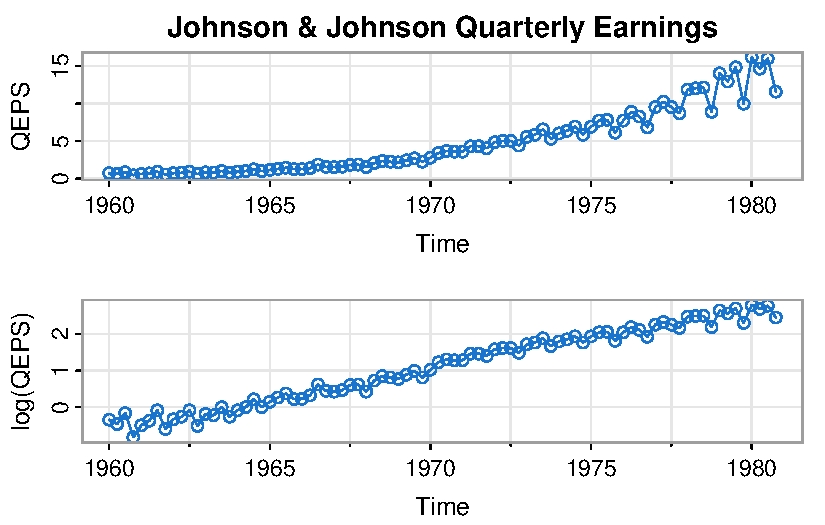
\includegraphics{LectureNotes/Lecture1_files/figure-pdf/ex-1-1-1.pdf}

\section{Example 1.2 (Climate Change)}\label{example-1.2-climate-change}

\begin{Shaded}
\begin{Highlighting}[]
\FunctionTok{tsplot}\NormalTok{(}\FunctionTok{cbind}\NormalTok{(gtemp\_land,gtemp\_ocean), }\AttributeTok{spaghetti=}\ConstantTok{TRUE}\NormalTok{, }\AttributeTok{col =} \FunctionTok{astsa.col}\NormalTok{(}\FunctionTok{c}\NormalTok{(}\DecValTok{2}\NormalTok{,}\DecValTok{4}\NormalTok{), .}\DecValTok{5}\NormalTok{), }
        \AttributeTok{lwd=}\DecValTok{2}\NormalTok{, }\AttributeTok{type=}\StringTok{"o"}\NormalTok{, }\AttributeTok{pch=}\DecValTok{20}\NormalTok{, }\AttributeTok{ylab=}\StringTok{"Temperature Deviations"}\NormalTok{, }\AttributeTok{main=}\StringTok{"Global Warming"}\NormalTok{)}
\FunctionTok{legend}\NormalTok{(}\StringTok{"topleft"}\NormalTok{, }\AttributeTok{col=}\FunctionTok{c}\NormalTok{(}\DecValTok{2}\NormalTok{,}\DecValTok{4}\NormalTok{), }\AttributeTok{lty=}\DecValTok{1}\NormalTok{, }\AttributeTok{lwd=}\DecValTok{2}\NormalTok{, }\AttributeTok{pch=}\DecValTok{20}\NormalTok{,  }\AttributeTok{bg=}\StringTok{"white"}\NormalTok{,}
        \AttributeTok{legend=}\FunctionTok{c}\NormalTok{(}\StringTok{"Land Surface"}\NormalTok{, }\StringTok{"Sea Surface"}\NormalTok{))}
\end{Highlighting}
\end{Shaded}

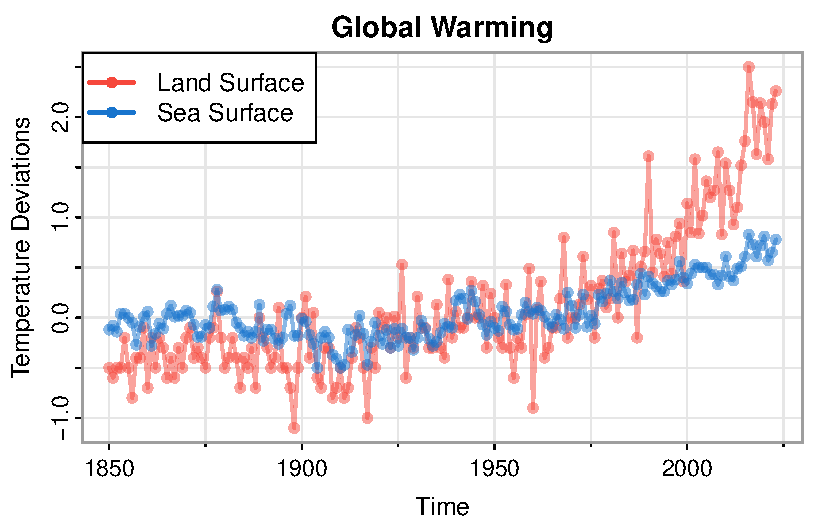
\includegraphics{LectureNotes/Lecture1_files/figure-pdf/ex-1-2-1.pdf}

\section{\texorpdfstring{{Example 1.3 (Dow Jones Industrial
Average)}}{Example 1.3 (Dow Jones Industrial Average)}}\label{example-1.3-dow-jones-industrial-average}

\begin{Shaded}
\begin{Highlighting}[]
\FunctionTok{library}\NormalTok{(xts)     }\CommentTok{\# install.packages("xts") if you don\textquotesingle{}t have it already }
\end{Highlighting}
\end{Shaded}

\begin{verbatim}
Loading required package: zoo
\end{verbatim}

\begin{verbatim}

Attaching package: 'zoo'
\end{verbatim}

\begin{verbatim}
The following objects are masked from 'package:base':

    as.Date, as.Date.numeric
\end{verbatim}

\begin{Shaded}
\begin{Highlighting}[]
\NormalTok{djia\_return }\OtherTok{=} \FunctionTok{diff}\NormalTok{(}\FunctionTok{log}\NormalTok{(djia}\SpecialCharTok{$}\NormalTok{Close))[}\SpecialCharTok{{-}}\DecValTok{1}\NormalTok{]}
\CommentTok{\#par(mfrow=2:1)}
\FunctionTok{plot}\NormalTok{(djia}\SpecialCharTok{$}\NormalTok{Close, }\AttributeTok{col=}\DecValTok{4}\NormalTok{)}
\end{Highlighting}
\end{Shaded}

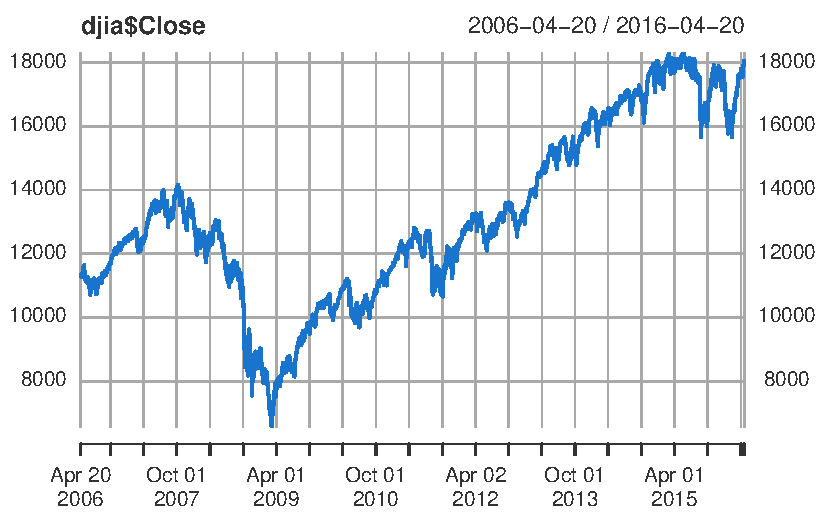
\includegraphics{LectureNotes/Lecture1_files/figure-pdf/ex-1-3-1.pdf}

\begin{Shaded}
\begin{Highlighting}[]
\FunctionTok{plot}\NormalTok{(djia\_return, }\AttributeTok{col=}\DecValTok{4}\NormalTok{)}
\end{Highlighting}
\end{Shaded}

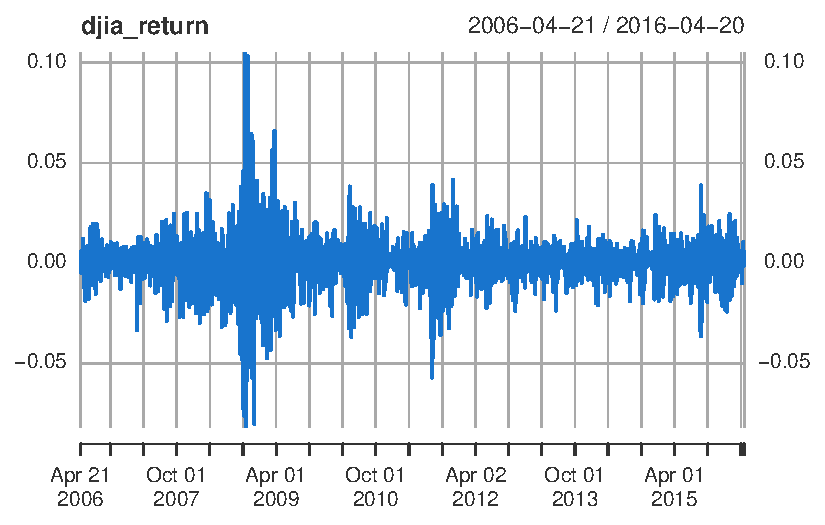
\includegraphics{LectureNotes/Lecture1_files/figure-pdf/ex-1-3-2.pdf}

\begin{Shaded}
\begin{Highlighting}[]
\FunctionTok{tsplot}\NormalTok{(}\FunctionTok{diff}\NormalTok{(}\FunctionTok{log}\NormalTok{(gdp)), }\AttributeTok{type=}\StringTok{"o"}\NormalTok{, }\AttributeTok{col=}\DecValTok{4}\NormalTok{)       }\CommentTok{\# using diff log}
\FunctionTok{points}\NormalTok{(}\FunctionTok{diff}\NormalTok{(gdp)}\SpecialCharTok{/}\FunctionTok{lag}\NormalTok{(gdp,}\SpecialCharTok{{-}}\DecValTok{1}\NormalTok{), }\AttributeTok{pch=}\StringTok{"+"}\NormalTok{, }\AttributeTok{col=}\DecValTok{2}\NormalTok{) }\CommentTok{\# actual return}
\end{Highlighting}
\end{Shaded}

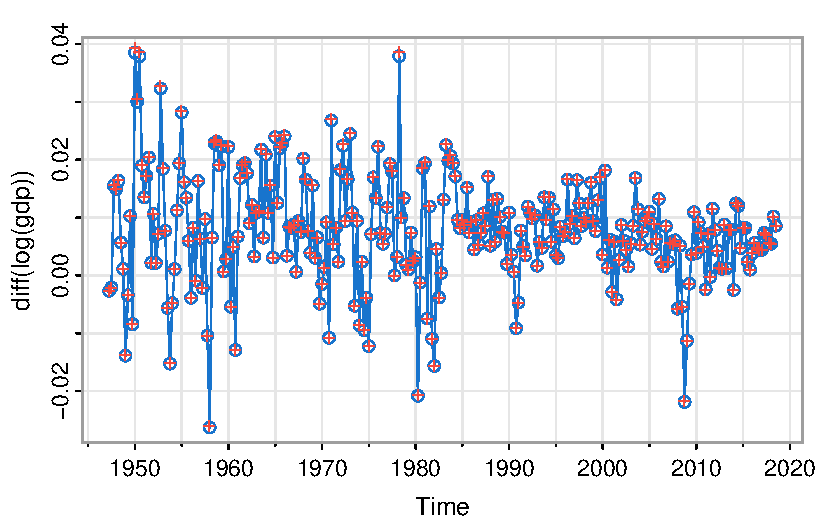
\includegraphics{LectureNotes/Lecture1_files/figure-pdf/ex-1-3-3.pdf}

\section{Example 1.4 El Niño}\label{example-1.4-el-niuxf1o}

\begin{Shaded}
\begin{Highlighting}[]
\FunctionTok{par}\NormalTok{(}\AttributeTok{mfrow =} \FunctionTok{c}\NormalTok{(}\DecValTok{2}\NormalTok{,}\DecValTok{1}\NormalTok{))}
\FunctionTok{tsplot}\NormalTok{(soi, }\AttributeTok{ylab=}\StringTok{""}\NormalTok{, }\AttributeTok{xlab=}\StringTok{""}\NormalTok{, }\AttributeTok{main=}\StringTok{"Southern Oscillation Index"}\NormalTok{, }\AttributeTok{col=}\DecValTok{4}\NormalTok{)}
\FunctionTok{text}\NormalTok{(}\DecValTok{1970}\NormalTok{, .}\DecValTok{91}\NormalTok{, }\StringTok{"COOL"}\NormalTok{, }\AttributeTok{col=}\DecValTok{5}\NormalTok{)}
\FunctionTok{text}\NormalTok{(}\DecValTok{1970}\NormalTok{,}\SpecialCharTok{{-}}\NormalTok{.}\DecValTok{91}\NormalTok{, }\StringTok{"WARM"}\NormalTok{, }\AttributeTok{col=}\DecValTok{6}\NormalTok{)}
\FunctionTok{tsplot}\NormalTok{(rec, }\AttributeTok{ylab=}\StringTok{""}\NormalTok{, }\AttributeTok{main=}\StringTok{"Recruitment"}\NormalTok{, }\AttributeTok{col=}\DecValTok{4}\NormalTok{) }
\end{Highlighting}
\end{Shaded}

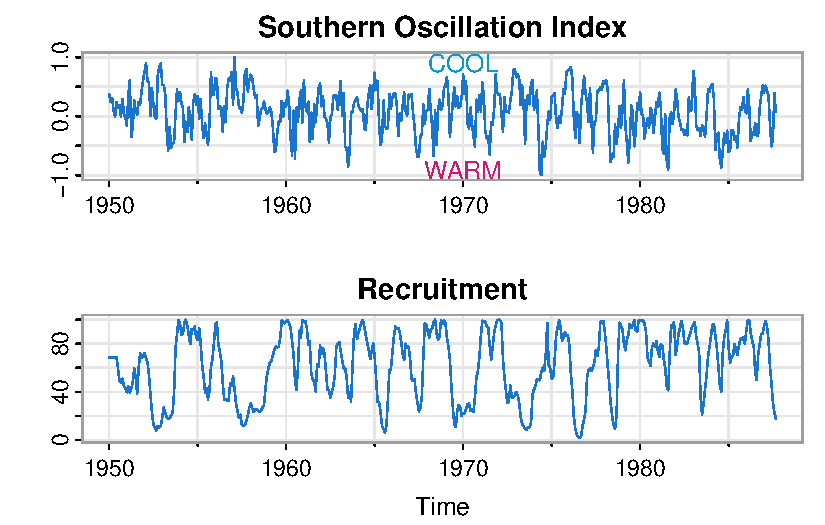
\includegraphics{LectureNotes/Lecture1_files/figure-pdf/ex-1-4-1.pdf}

\section{\texorpdfstring{{Example 1.5 (Predator-Prey
Interactions)}}{Example 1.5 (Predator-Prey Interactions)}}\label{example-1.5-predator-prey-interactions}

\href{https://www.gov.nt.ca/ecc/en/services/lynx/lynx-snowshoe-hare-cycle}{Link
to more info!}

\begin{Shaded}
\begin{Highlighting}[]
\FunctionTok{tsplot}\NormalTok{(}\FunctionTok{cbind}\NormalTok{(Hare,Lynx), }\AttributeTok{col =} \FunctionTok{astsa.col}\NormalTok{(}\FunctionTok{c}\NormalTok{(}\DecValTok{2}\NormalTok{,}\DecValTok{4}\NormalTok{), .}\DecValTok{6}\NormalTok{), }\AttributeTok{lwd=}\DecValTok{2}\NormalTok{, }\AttributeTok{type=}\StringTok{"o"}\NormalTok{, }\AttributeTok{pch=}\FunctionTok{c}\NormalTok{(}\DecValTok{0}\NormalTok{,}\DecValTok{2}\NormalTok{),}
        \AttributeTok{spaghetti=}\ConstantTok{TRUE}\NormalTok{, }\AttributeTok{ylab=}\FunctionTok{expression}\NormalTok{(Number}\SpecialCharTok{\textasciitilde{}}\ErrorTok{\textasciitilde{}\textasciitilde{}}\NormalTok{(}\StringTok{""}\SpecialCharTok{\%*\%} \DecValTok{1000}\NormalTok{)))}
\FunctionTok{legend}\NormalTok{(}\StringTok{"topright"}\NormalTok{, }\AttributeTok{col=}\FunctionTok{c}\NormalTok{(}\DecValTok{2}\NormalTok{,}\DecValTok{4}\NormalTok{), }\AttributeTok{lty=}\DecValTok{1}\NormalTok{, }\AttributeTok{lwd=}\DecValTok{2}\NormalTok{, }\AttributeTok{pch=}\FunctionTok{c}\NormalTok{(}\DecValTok{0}\NormalTok{,}\DecValTok{2}\NormalTok{), }\AttributeTok{legend=}\FunctionTok{c}\NormalTok{(}\StringTok{"Hare"}\NormalTok{, }\StringTok{"Lynx"}\NormalTok{), }\AttributeTok{bty=}\StringTok{"n"}\NormalTok{)}
\end{Highlighting}
\end{Shaded}

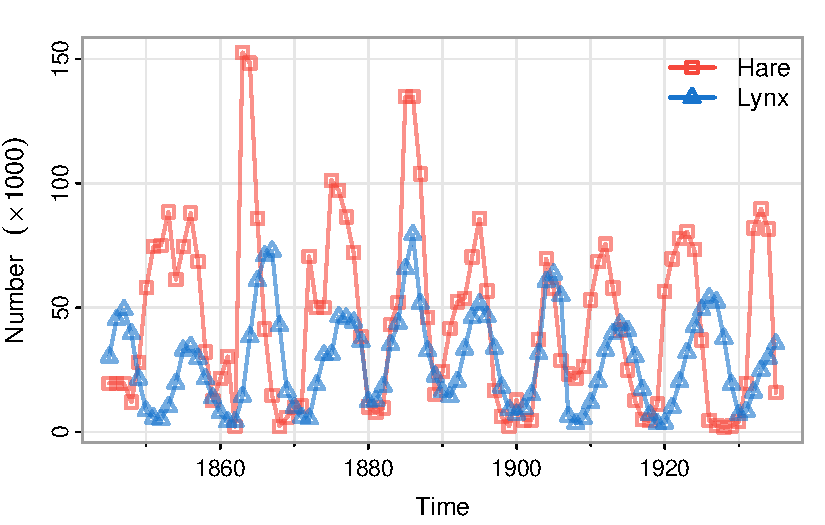
\includegraphics{LectureNotes/Lecture1_files/figure-pdf/ex-1-5-1.pdf}

\subsection{Cute animal pictures}\label{cute-animal-pictures}

\includegraphics{index_files/mediabag/1000_F_237306331_HH4.jpg}

\includegraphics{index_files/mediabag/20191230-img-hare_or.jpg}

\includegraphics{index_files/mediabag/lynx.jpg}

\section{Example 1.6 fMRI Imaging}\label{example-1.6-fmri-imaging}

\begin{Shaded}
\begin{Highlighting}[]
\FunctionTok{par}\NormalTok{(}\AttributeTok{mfrow=}\FunctionTok{c}\NormalTok{(}\DecValTok{3}\NormalTok{,}\DecValTok{1}\NormalTok{))}
\NormalTok{x }\OtherTok{=} \FunctionTok{ts}\NormalTok{(fmri1[,}\DecValTok{4}\SpecialCharTok{:}\DecValTok{9}\NormalTok{], }\AttributeTok{start=}\DecValTok{0}\NormalTok{, }\AttributeTok{freq=}\DecValTok{32}\NormalTok{)        }\CommentTok{\# data}
\NormalTok{names }\OtherTok{=} \FunctionTok{c}\NormalTok{(}\StringTok{"Cortex"}\NormalTok{,}\StringTok{"Thalamus"}\NormalTok{,}\StringTok{"Cerebellum"}\NormalTok{)}
\NormalTok{u }\OtherTok{=} \FunctionTok{ts}\NormalTok{(}\FunctionTok{rep}\NormalTok{(}\FunctionTok{c}\NormalTok{(}\FunctionTok{rep}\NormalTok{(.}\DecValTok{6}\NormalTok{,}\DecValTok{16}\NormalTok{), }\FunctionTok{rep}\NormalTok{(}\SpecialCharTok{{-}}\NormalTok{.}\DecValTok{6}\NormalTok{,}\DecValTok{16}\NormalTok{)), }\DecValTok{4}\NormalTok{), }\AttributeTok{start=}\DecValTok{0}\NormalTok{, }\AttributeTok{freq=}\DecValTok{32}\NormalTok{) }\CommentTok{\# stimulus signal}

\ControlFlowTok{for}\NormalTok{ (i }\ControlFlowTok{in} \DecValTok{1}\SpecialCharTok{:}\DecValTok{3}\NormalTok{)\{ }
\NormalTok{ j }\OtherTok{=} \DecValTok{2}\SpecialCharTok{*}\NormalTok{i}\DecValTok{{-}1}
 \FunctionTok{tsplot}\NormalTok{(x[,j}\SpecialCharTok{:}\NormalTok{(j}\SpecialCharTok{+}\DecValTok{1}\NormalTok{)], }\AttributeTok{ylab=}\StringTok{"BOLD"}\NormalTok{, }\AttributeTok{xlab=}\StringTok{""}\NormalTok{, }\AttributeTok{main=}\NormalTok{names[i], }\AttributeTok{col=}\DecValTok{5}\SpecialCharTok{:}\DecValTok{6}\NormalTok{, }\AttributeTok{ylim=}\FunctionTok{c}\NormalTok{(}\SpecialCharTok{{-}}\NormalTok{.}\DecValTok{6}\NormalTok{,.}\DecValTok{6}\NormalTok{), }
        \AttributeTok{lwd=}\DecValTok{2}\NormalTok{, }\AttributeTok{xaxt=}\StringTok{"n"}\NormalTok{, }\AttributeTok{spaghetti=}\ConstantTok{TRUE}\NormalTok{)}
 \FunctionTok{axis}\NormalTok{(}\FunctionTok{seq}\NormalTok{(}\DecValTok{0}\NormalTok{,}\DecValTok{256}\NormalTok{,}\DecValTok{64}\NormalTok{), }\AttributeTok{side=}\DecValTok{1}\NormalTok{, }\AttributeTok{at=}\DecValTok{0}\SpecialCharTok{:}\DecValTok{4}\NormalTok{)}
 \CommentTok{\#lines(u, type="s", col=gray(.3)) }
\NormalTok{\}}
\FunctionTok{mtext}\NormalTok{(}\StringTok{"seconds"}\NormalTok{, }\AttributeTok{side=}\DecValTok{1}\NormalTok{, }\AttributeTok{line=}\FloatTok{1.75}\NormalTok{, }\AttributeTok{cex=}\NormalTok{.}\DecValTok{9}\NormalTok{)}
\end{Highlighting}
\end{Shaded}

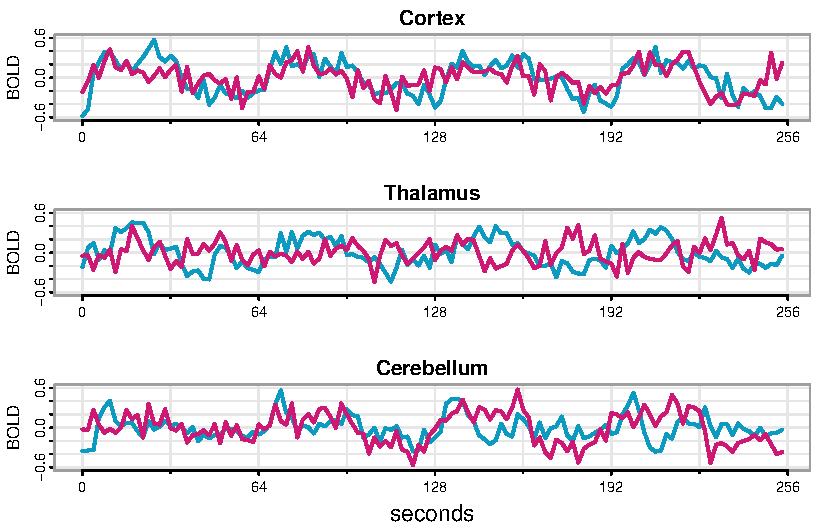
\includegraphics{LectureNotes/Lecture1_files/figure-pdf/ex-1-6-no-lines-1.pdf}

\begin{Shaded}
\begin{Highlighting}[]
\FunctionTok{par}\NormalTok{(}\AttributeTok{mfrow=}\FunctionTok{c}\NormalTok{(}\DecValTok{3}\NormalTok{,}\DecValTok{1}\NormalTok{))}
\NormalTok{x }\OtherTok{=} \FunctionTok{ts}\NormalTok{(fmri1[,}\DecValTok{4}\SpecialCharTok{:}\DecValTok{9}\NormalTok{], }\AttributeTok{start=}\DecValTok{0}\NormalTok{, }\AttributeTok{freq=}\DecValTok{32}\NormalTok{)        }\CommentTok{\# data}
\NormalTok{names }\OtherTok{=} \FunctionTok{c}\NormalTok{(}\StringTok{"Cortex"}\NormalTok{,}\StringTok{"Thalamus"}\NormalTok{,}\StringTok{"Cerebellum"}\NormalTok{)}
\NormalTok{u }\OtherTok{=} \FunctionTok{ts}\NormalTok{(}\FunctionTok{rep}\NormalTok{(}\FunctionTok{c}\NormalTok{(}\FunctionTok{rep}\NormalTok{(.}\DecValTok{6}\NormalTok{,}\DecValTok{16}\NormalTok{), }\FunctionTok{rep}\NormalTok{(}\SpecialCharTok{{-}}\NormalTok{.}\DecValTok{6}\NormalTok{,}\DecValTok{16}\NormalTok{)), }\DecValTok{4}\NormalTok{), }\AttributeTok{start=}\DecValTok{0}\NormalTok{, }\AttributeTok{freq=}\DecValTok{32}\NormalTok{) }\CommentTok{\# stimulus signal}

\ControlFlowTok{for}\NormalTok{ (i }\ControlFlowTok{in} \DecValTok{1}\SpecialCharTok{:}\DecValTok{3}\NormalTok{)\{ }
\NormalTok{ j }\OtherTok{=} \DecValTok{2}\SpecialCharTok{*}\NormalTok{i}\DecValTok{{-}1}
 \FunctionTok{tsplot}\NormalTok{(x[,j}\SpecialCharTok{:}\NormalTok{(j}\SpecialCharTok{+}\DecValTok{1}\NormalTok{)], }\AttributeTok{ylab=}\StringTok{"BOLD"}\NormalTok{, }\AttributeTok{xlab=}\StringTok{""}\NormalTok{, }\AttributeTok{main=}\NormalTok{names[i], }\AttributeTok{col=}\DecValTok{5}\SpecialCharTok{:}\DecValTok{6}\NormalTok{, }\AttributeTok{ylim=}\FunctionTok{c}\NormalTok{(}\SpecialCharTok{{-}}\NormalTok{.}\DecValTok{6}\NormalTok{,.}\DecValTok{6}\NormalTok{), }
        \AttributeTok{lwd=}\DecValTok{2}\NormalTok{, }\AttributeTok{xaxt=}\StringTok{"n"}\NormalTok{, }\AttributeTok{spaghetti=}\ConstantTok{TRUE}\NormalTok{)}
 \FunctionTok{axis}\NormalTok{(}\FunctionTok{seq}\NormalTok{(}\DecValTok{0}\NormalTok{,}\DecValTok{256}\NormalTok{,}\DecValTok{64}\NormalTok{), }\AttributeTok{side=}\DecValTok{1}\NormalTok{, }\AttributeTok{at=}\DecValTok{0}\SpecialCharTok{:}\DecValTok{4}\NormalTok{)}
 \FunctionTok{lines}\NormalTok{(u, }\AttributeTok{type=}\StringTok{"s"}\NormalTok{, }\AttributeTok{col=}\FunctionTok{gray}\NormalTok{(.}\DecValTok{3}\NormalTok{)) }
\NormalTok{\}}
\FunctionTok{mtext}\NormalTok{(}\StringTok{"seconds"}\NormalTok{, }\AttributeTok{side=}\DecValTok{1}\NormalTok{, }\AttributeTok{line=}\FloatTok{1.75}\NormalTok{, }\AttributeTok{cex=}\NormalTok{.}\DecValTok{9}\NormalTok{)}
\end{Highlighting}
\end{Shaded}

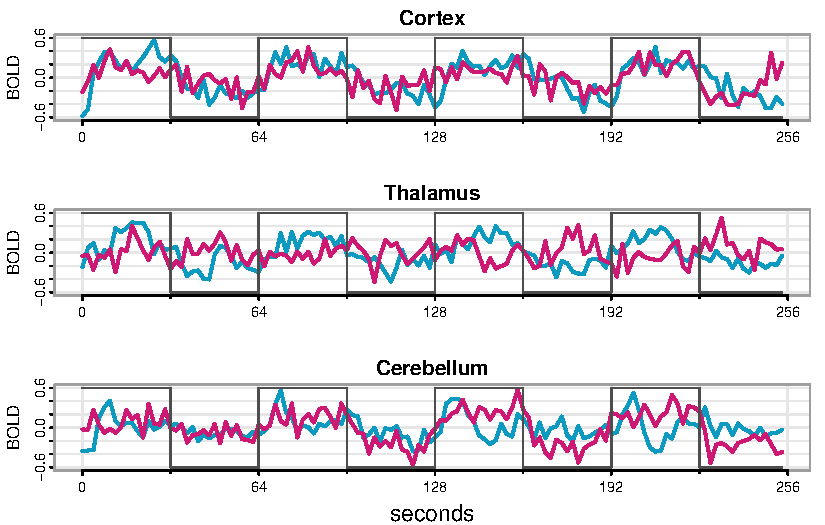
\includegraphics{LectureNotes/Lecture1_files/figure-pdf/ex-1-6-1.pdf}

\chapter{Introduction to Time Series
Models}\label{introduction-to-time-series-models}

\section{White Noise}\label{white-noise}

\begin{itemize}
\item
  in general, a collection of random variables \(w_t\)

  \begin{itemize}
  \item
    uncorrelated
  \item
    mean 0, variance \(\sigma_w^2\)
  \item
    denoted \(w_t \sim wn(0, \sigma_w^2)\)
  \end{itemize}
\item
  for us, usually independent and identically distributed (i.i.d.)
  normal

  \begin{itemize}
  \tightlist
  \item
    \(w_t \sim \text{iid } N(0, \sigma_w^2)\)
  \end{itemize}
\end{itemize}

\section{Plotting White Noise}\label{plotting-white-noise}

Which example does this bear the most resemblance to?

\begin{Shaded}
\begin{Highlighting}[]
\NormalTok{w }\OtherTok{\textless{}{-}} \FunctionTok{rnorm}\NormalTok{(}\DecValTok{500}\NormalTok{, }\DecValTok{0}\NormalTok{, }\DecValTok{1}\NormalTok{)}
\FunctionTok{plot}\NormalTok{(w, }\AttributeTok{type =} \StringTok{"p"}\NormalTok{, }\AttributeTok{col =} \StringTok{"blue"}\NormalTok{, }\AttributeTok{xlab =} \StringTok{"t (order of sampling)"}\NormalTok{)}
\end{Highlighting}
\end{Shaded}

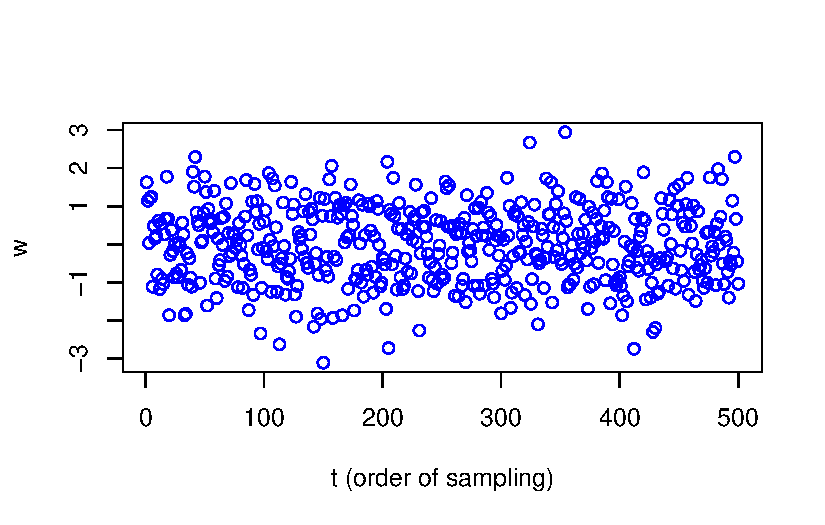
\includegraphics{LectureNotes/Lecture1_files/figure-pdf/white-noise-1.pdf}

\section{\texorpdfstring{What White Noise
\emph{isn't}}{What White Noise isn't}}\label{what-white-noise-isnt}

\begin{itemize}
\item
  serially correlated -- no temporal structure
\item
  smooth -- ``nice'' trend/temporal structure
\end{itemize}

How can we build this ``nice'' structure into the model?

\section{\texorpdfstring{{Moving Averages, Smoothing, and
Filtering}}{Moving Averages, Smoothing, and Filtering}}\label{moving-averages-smoothing-and-filtering}

Replace \(w_t\) with an average of its current value and two previous
values:

\[
v_t = \frac{1}{3}(w_{t-2} + w_{t-1} + w_{t})
\]

\begin{itemize}
\item
  Why do we divide by 3?
\item
  If \(w_t \sim \text{iid } N(0, \sigma_w^2)\), what is the distribution
  of \(v_t\)?
\item
  Why only the previous two values? Why not one in the past and one in
  the future?
\end{itemize}

\section{Plotting a Moving Average}\label{plotting-a-moving-average}

\begin{Shaded}
\begin{Highlighting}[]
\NormalTok{v }\OtherTok{=}\NormalTok{ stats}\SpecialCharTok{::}\FunctionTok{filter}\NormalTok{(w, }\AttributeTok{sides =} \DecValTok{2}\NormalTok{, }\AttributeTok{filter =} \FunctionTok{rep}\NormalTok{(}\DecValTok{1}\SpecialCharTok{/}\DecValTok{3}\NormalTok{, }\DecValTok{3}\NormalTok{))}
\NormalTok{v\_alt }\OtherTok{=}\NormalTok{ stats}\SpecialCharTok{::}\FunctionTok{filter}\NormalTok{(w, }\AttributeTok{sides =} \DecValTok{1}\NormalTok{, }\AttributeTok{filter =} \FunctionTok{rep}\NormalTok{(}\DecValTok{1}\SpecialCharTok{/}\DecValTok{3}\NormalTok{,}\DecValTok{3}\NormalTok{))}
\FunctionTok{par}\NormalTok{(}\AttributeTok{mfrow=}\DecValTok{2}\SpecialCharTok{:}\DecValTok{1}\NormalTok{)}
\FunctionTok{tsplot}\NormalTok{(v, }\AttributeTok{ylim =} \FunctionTok{c}\NormalTok{(}\SpecialCharTok{{-}}\DecValTok{3}\NormalTok{, }\DecValTok{3}\NormalTok{), }\AttributeTok{col =} \DecValTok{4}\NormalTok{, }\AttributeTok{main=}\StringTok{"moving average"}\NormalTok{)}
\FunctionTok{tsplot}\NormalTok{(v\_alt, }\AttributeTok{ylim =} \FunctionTok{c}\NormalTok{(}\SpecialCharTok{{-}}\DecValTok{3}\NormalTok{, }\DecValTok{3}\NormalTok{), }\AttributeTok{col =} \DecValTok{4}\NormalTok{, }\AttributeTok{main=}\StringTok{"moving average"}\NormalTok{)}
\end{Highlighting}
\end{Shaded}

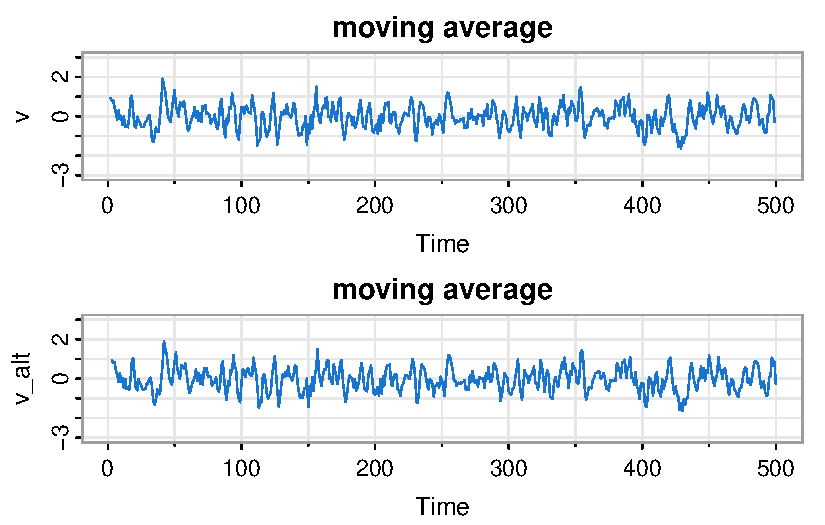
\includegraphics{LectureNotes/Lecture1_files/figure-pdf/moving-average-1.pdf}

Compare this moving average to the SOI and Recruitment series. How do
they differ?

\section{Autoregressions}\label{autoregressions}

Starting with white noise \(w_t\), consider the equation:

\[
x_t = 1.5x_{t-1} - 0.75x_{t-2} + w_t
\]

\begin{itemize}
\item
  a ``second-order equation'' (why?)
\item
  A regression of the current value \(x_t\) of a time series as a
  function of the past two values of the series

  \begin{itemize}
  \item
    \href{https://www.merriam-webster.com/dictionary/auto}{``auto''
    means self}
  \item
    recall (multiple) regression of \(Y\) on \(X = (X_1, X_2)\) is
    \(Y = \beta_0 + \beta_1X_1 + \beta_2X_2 + \varepsilon\) and compare
    to autoregression formula above
  \item
    See (or hear) details in textbook page 11
  \end{itemize}
\end{itemize}

\section{Plotting Autoregressions}\label{plotting-autoregressions}

\begin{Shaded}
\begin{Highlighting}[]
\FunctionTok{set.seed}\NormalTok{(}\DecValTok{90210}\NormalTok{)}
\NormalTok{w }\OtherTok{=} \FunctionTok{rnorm}\NormalTok{(}\DecValTok{250} \SpecialCharTok{+} \DecValTok{50}\NormalTok{) }\CommentTok{\# 50 extra to avoid startup problems}
\NormalTok{x }\OtherTok{=} \FunctionTok{filter}\NormalTok{(w, }\AttributeTok{filter=}\FunctionTok{c}\NormalTok{(}\FloatTok{1.5}\NormalTok{,}\SpecialCharTok{{-}}\NormalTok{.}\DecValTok{75}\NormalTok{), }\AttributeTok{method=}\StringTok{"recursive"}\NormalTok{)[}\SpecialCharTok{{-}}\NormalTok{(}\DecValTok{1}\SpecialCharTok{:}\DecValTok{50}\NormalTok{)]}
\FunctionTok{tsplot}\NormalTok{(x, }\AttributeTok{main=}\StringTok{"autoregression"}\NormalTok{, }\AttributeTok{col=}\DecValTok{4}\NormalTok{)}
\end{Highlighting}
\end{Shaded}

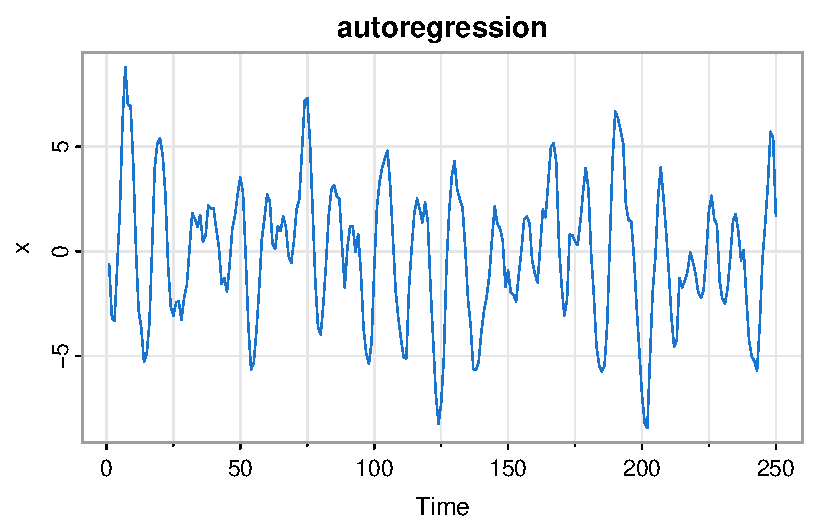
\includegraphics{LectureNotes/Lecture1_files/figure-pdf/autoregressions-1.pdf}

\section{Random Walk with Drift}\label{random-walk-with-drift}

Again starting with white noise \(w_t \sim wn(0, \sigma^2_2)\), consider
the time series

\[
x_t = \delta + x_{t-1} + w_t
\]

This is called the ``random walk with drift'' model.

\begin{itemize}
\item
  \(\delta\) is the drift term (\(\delta = 0\) corresponds to ``random
  walk''- no drift)
\item
  initial condition \(x_0 = 0\)
\end{itemize}

Can be rewritten

\[
x_t = \delta t + \sum_{j=1}^t w_j
\]

\section{Plotting a Random Walk with
Drift}\label{plotting-a-random-walk-with-drift}

\begin{Shaded}
\begin{Highlighting}[]
\FunctionTok{set.seed}\NormalTok{(}\DecValTok{314159265}\NormalTok{) }\CommentTok{\# so you can reproduce the results}
\NormalTok{w  }\OtherTok{=} \FunctionTok{rnorm}\NormalTok{(}\DecValTok{200}\NormalTok{)  }\DocumentationTok{\#\# Gaussian white noise}
\NormalTok{x  }\OtherTok{=} \FunctionTok{cumsum}\NormalTok{(w)}
\NormalTok{wd }\OtherTok{=}\NormalTok{ w }\SpecialCharTok{+}\NormalTok{.}\DecValTok{3} 
\NormalTok{xd }\OtherTok{=} \FunctionTok{cumsum}\NormalTok{(wd)}
\FunctionTok{tsplot}\NormalTok{(xd, }\AttributeTok{ylim=}\FunctionTok{c}\NormalTok{(}\SpecialCharTok{{-}}\DecValTok{2}\NormalTok{,}\DecValTok{80}\NormalTok{), }\AttributeTok{main=}\StringTok{"random walk"}\NormalTok{, }\AttributeTok{ylab=}\StringTok{""}\NormalTok{, }\AttributeTok{col=}\DecValTok{4}\NormalTok{)}
 \FunctionTok{clip}\NormalTok{(}\DecValTok{0}\NormalTok{, }\DecValTok{200}\NormalTok{, }\DecValTok{0}\NormalTok{, }\DecValTok{80}\NormalTok{)}
 \FunctionTok{abline}\NormalTok{(}\AttributeTok{a=}\DecValTok{0}\NormalTok{, }\AttributeTok{b=}\NormalTok{.}\DecValTok{3}\NormalTok{, }\AttributeTok{lty=}\DecValTok{2}\NormalTok{, }\AttributeTok{col=}\DecValTok{4}\NormalTok{) }\CommentTok{\# drift}
\FunctionTok{lines}\NormalTok{(x, }\AttributeTok{col=}\DecValTok{6}\NormalTok{)}
 \FunctionTok{clip}\NormalTok{(}\DecValTok{0}\NormalTok{, }\DecValTok{200}\NormalTok{, }\DecValTok{0}\NormalTok{, }\DecValTok{80}\NormalTok{)}
 \FunctionTok{abline}\NormalTok{(}\AttributeTok{h=}\DecValTok{0}\NormalTok{, }\AttributeTok{col=}\DecValTok{6}\NormalTok{, }\AttributeTok{lty=}\DecValTok{2}\NormalTok{)}
\end{Highlighting}
\end{Shaded}

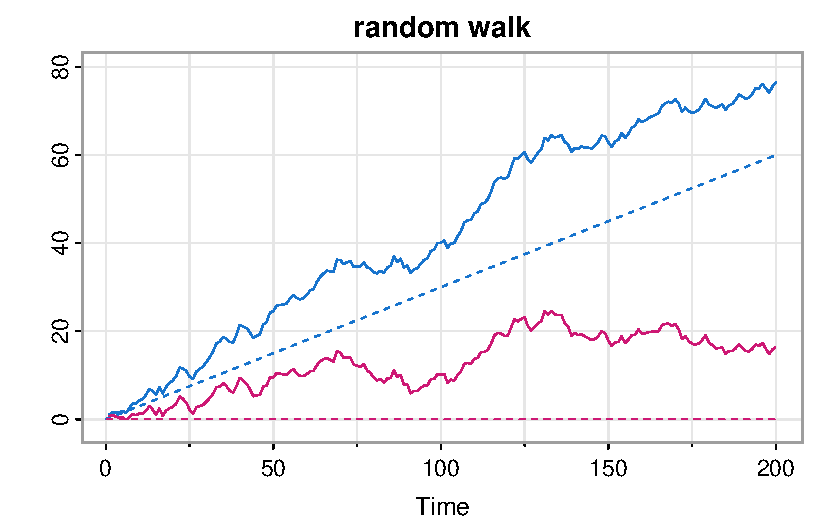
\includegraphics{LectureNotes/Lecture1_files/figure-pdf/random-walk-with-drift-1.pdf}

\section{Signal Plus Noise}\label{signal-plus-noise}

Consider the model:

\[
x_t = 2\cos(2\pi\frac{t + 15}{50}) + w_t
\]

\begin{itemize}
\item
  \(2\cos(2\pi\frac{t + 15}{50})\) is the signal
\item
  \(w_t\) is the noise
\end{itemize}

\section{\texorpdfstring{{Plotting Signal Plus Noise (two
scenarios)}}{Plotting Signal Plus Noise (two scenarios)}}\label{plotting-signal-plus-noise-two-scenarios}

\begin{Shaded}
\begin{Highlighting}[]
\CommentTok{\# cs = 2*cos(2*pi*(1:500)/50 + .6*pi)    \# as in the text}
\NormalTok{cs }\OtherTok{=} \DecValTok{2}\SpecialCharTok{*}\FunctionTok{cos}\NormalTok{(}\DecValTok{2}\SpecialCharTok{*}\NormalTok{pi}\SpecialCharTok{*}\NormalTok{(}\DecValTok{1}\SpecialCharTok{:}\DecValTok{500}\SpecialCharTok{+}\DecValTok{15}\NormalTok{)}\SpecialCharTok{/}\DecValTok{50}\NormalTok{)           }\CommentTok{\# same thing }
\NormalTok{w  }\OtherTok{=} \FunctionTok{rnorm}\NormalTok{(}\DecValTok{500}\NormalTok{,}\DecValTok{0}\NormalTok{,}\DecValTok{1}\NormalTok{)}
\FunctionTok{par}\NormalTok{(}\AttributeTok{mfrow=}\FunctionTok{c}\NormalTok{(}\DecValTok{3}\NormalTok{,}\DecValTok{1}\NormalTok{))   }
\FunctionTok{tsplot}\NormalTok{(cs, }\AttributeTok{ylab=}\StringTok{""}\NormalTok{, }\AttributeTok{main =} \FunctionTok{expression}\NormalTok{(x[t]}\SpecialCharTok{==}\DecValTok{2}\SpecialCharTok{*}\FunctionTok{cos}\NormalTok{(}\DecValTok{2}\SpecialCharTok{*}\NormalTok{pi}\SpecialCharTok{*}\NormalTok{t}\SpecialCharTok{/}\DecValTok{50}\FloatTok{+.6}\SpecialCharTok{*}\NormalTok{pi)))}
\FunctionTok{tsplot}\NormalTok{(cs }\SpecialCharTok{+}\NormalTok{ w, }\AttributeTok{ylab=}\StringTok{""}\NormalTok{, }\AttributeTok{main =} \FunctionTok{expression}\NormalTok{(x[t]}\SpecialCharTok{==}\DecValTok{2}\SpecialCharTok{*}\FunctionTok{cos}\NormalTok{(}\DecValTok{2}\SpecialCharTok{*}\NormalTok{pi}\SpecialCharTok{*}\NormalTok{t}\SpecialCharTok{/}\DecValTok{50}\FloatTok{+.6}\SpecialCharTok{*}\NormalTok{pi)}\SpecialCharTok{+}\FunctionTok{N}\NormalTok{(}\DecValTok{0}\NormalTok{,}\DecValTok{1}\NormalTok{)))}
\FunctionTok{tsplot}\NormalTok{(cs }\SpecialCharTok{+} \DecValTok{5}\SpecialCharTok{*}\NormalTok{w, }\AttributeTok{ylab=}\StringTok{""}\NormalTok{, }\AttributeTok{main =} \FunctionTok{expression}\NormalTok{(x[t]}\SpecialCharTok{==}\DecValTok{2}\SpecialCharTok{*}\FunctionTok{cos}\NormalTok{(}\DecValTok{2}\SpecialCharTok{*}\NormalTok{pi}\SpecialCharTok{*}\NormalTok{t}\SpecialCharTok{/}\DecValTok{50}\FloatTok{+.6}\SpecialCharTok{*}\NormalTok{pi)}\SpecialCharTok{+}\FunctionTok{N}\NormalTok{(}\DecValTok{0}\NormalTok{,}\DecValTok{25}\NormalTok{)))}
\end{Highlighting}
\end{Shaded}

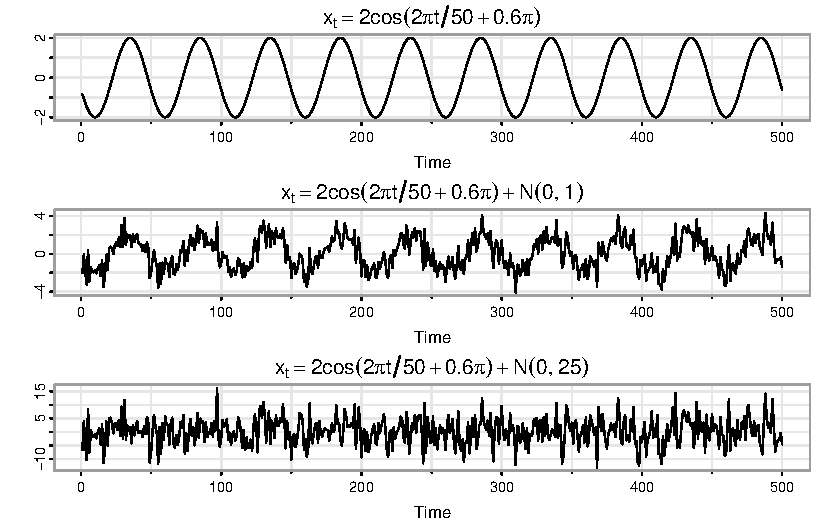
\includegraphics{LectureNotes/Lecture1_files/figure-pdf/signal-plus-noise-1.pdf}

\section{Next Time}\label{next-time}

\begin{itemize}
\item
  Exercises at the end of chapter 1
\item
  Start Chapter 2

  \begin{itemize}
  \tightlist
  \item
    Review definition of covariance, correlation, expected value, and
    variance (good use of AI-- prompt then Wikipedia?)
  \end{itemize}
\end{itemize}

\chapter{Lecture 2}\label{lecture-2}

\[
\newcommand\E{{\mathbb{E}}}
\]

\section{Recap from last time}\label{recap-from-last-time}

\begin{itemize}
\item
  Several examples of time series data sets
\item
  Experience plotting the time series
\item
  Exposure to some common time series models
\end{itemize}

\section{Today}\label{today}

\begin{itemize}
\tightlist
\item
  Notation review
\item
  Mean and covariance function of a time series
\item
  R code activity
\item
  Stationarity (if time)
\end{itemize}

\section{Coming up/notices}\label{coming-upnotices}

\begin{itemize}
\tightlist
\item
  I combined the Canvas sections (applies to section 2)
\item
  Quiz 1 posted today, due tomorrow at midnight (20 minutes to do it)
\item
  Assignment 1 will also be posted today, due Monday at midnight
  (boundary between Monday and Tuesday)
\item
  Next week's office hours: M 4-5, T 12-2
\end{itemize}

\chapter{Review of notation}\label{review-of-notation}

\section{Notation and Data- White
noise}\label{notation-and-data--white-noise}

``Let \(w_t\) be a white noise series''

\begin{longtable}[]{@{}lll@{}}
\toprule\noalign{}
t & Random Variable & Example data \\
\midrule\noalign{}
\endhead
\bottomrule\noalign{}
\endlastfoot
1 & \(w_1 \sim N(0, \sigma_w^2)\) & -0.0777401 \\
2 & \(w_2 \sim N(0, \sigma_w^2)\) & -1.2742499 \\
& \(\vdots\) & \(\vdots\) \\
t & \(w_t \sim N(0, \sigma^2_w)\) & -0.3434436 \\
\(\vdots\) & \(\vdots\) & \(\vdots\) \\
n & \(w_n \sim N(0, \sigma_w^2)\) & 0.068451 \\
\end{longtable}

If we interpret the collection of \(w_t\) as a random vector, then
\(w_t \sim MVN(\vec{0}, I)\) (why \(I\)?)

Note: sometimes \(w_t\) could mean a (univariate) value of a white noise
series for a particular time \(t\) (kind of like how you refer to an
arbitrary \(x_i\) when you have a sample \(x_1, \dots, x_n\)).

\section{\texorpdfstring{{(Aside) The Multivariate normal
distribution}}{(Aside) The Multivariate normal distribution}}\label{aside-the-multivariate-normal-distribution}

Let's look on
\href{https://en.wikipedia.org/wiki/Multivariate_normal_distribution}{Wikipedia}.
What are the parameters?

\begin{itemize}
\item
  mean \textbf{vector}
\item
  variance (covariance) \textbf{matrix}

  \begin{itemize}
  \tightlist
  \item
    If the covariance matrix is the identity matrix, the the covariances
    are 0
  \end{itemize}
\end{itemize}

\section{\texorpdfstring{{(Aside) Bivariate normal distribution for
uncorrelated
case}}{(Aside) Bivariate normal distribution for uncorrelated case}}\label{aside-bivariate-normal-distribution-for-uncorrelated-case}

\begin{Shaded}
\begin{Highlighting}[]
\CommentTok{\# install.packages("ggplot2")}
\CommentTok{\# install.packages("ggExtra")}
\FunctionTok{library}\NormalTok{(ggplot2)}
\FunctionTok{library}\NormalTok{(ggExtra)}

\NormalTok{x1 }\OtherTok{\textless{}{-}} \FunctionTok{rnorm}\NormalTok{(}\DecValTok{100}\NormalTok{, }\DecValTok{10}\NormalTok{, }\DecValTok{5}\NormalTok{)}
\NormalTok{x2 }\OtherTok{\textless{}{-}} \FunctionTok{rnorm}\NormalTok{(}\DecValTok{100}\NormalTok{, .}\DecValTok{1}\NormalTok{, .}\DecValTok{5}\NormalTok{)}

\NormalTok{x }\OtherTok{\textless{}{-}} \FunctionTok{data.frame}\NormalTok{(x1, x2)}
\CommentTok{\# Save the scatter plot in a variable}
\NormalTok{p }\OtherTok{\textless{}{-}} \FunctionTok{ggplot}\NormalTok{(x, }\FunctionTok{aes}\NormalTok{(}\AttributeTok{x =}\NormalTok{ x1, }\AttributeTok{y =}\NormalTok{ x2)) }\SpecialCharTok{+}
  \FunctionTok{geom\_point}\NormalTok{()}

\CommentTok{\# Arguments for each marginal histogram}
\FunctionTok{ggMarginal}\NormalTok{(p, }\AttributeTok{type =} \StringTok{"histogram"}\NormalTok{, }
           \AttributeTok{xparams =} \FunctionTok{list}\NormalTok{(}\AttributeTok{fill =} \DecValTok{4}\NormalTok{),}
           \AttributeTok{yparams =} \FunctionTok{list}\NormalTok{(}\AttributeTok{fill =} \DecValTok{3}\NormalTok{))}
\end{Highlighting}
\end{Shaded}

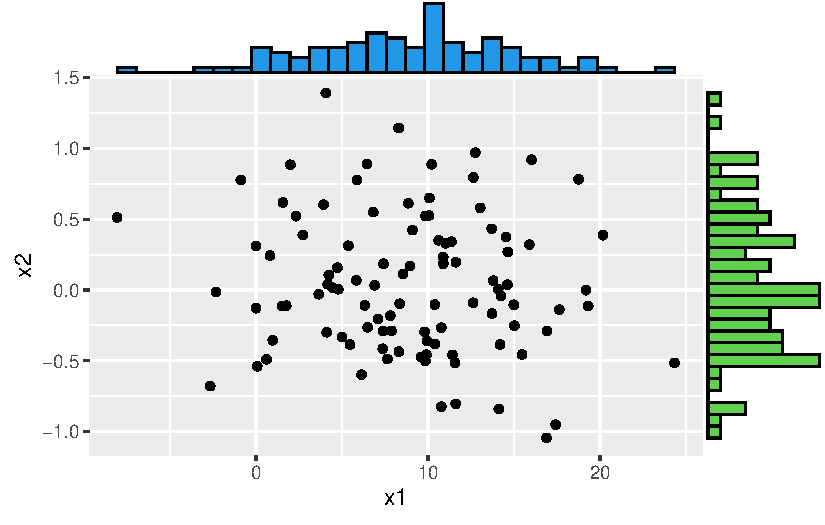
\includegraphics{LectureNotes/Lecture2_files/figure-pdf/unnamed-chunk-1-1.pdf}

\section{\texorpdfstring{{(Aside) Bivariate normal distribution for
correlated
case}}{(Aside) Bivariate normal distribution for correlated case}}\label{aside-bivariate-normal-distribution-for-correlated-case}

\begin{Shaded}
\begin{Highlighting}[]
\CommentTok{\#install.packages("MASS")}
\FunctionTok{library}\NormalTok{(MASS)}

\NormalTok{mu }\OtherTok{\textless{}{-}} \FunctionTok{c}\NormalTok{(}\DecValTok{10}\NormalTok{, .}\DecValTok{1}\NormalTok{)}
\NormalTok{varcov }\OtherTok{\textless{}{-}} \FunctionTok{matrix}\NormalTok{(}\FunctionTok{c}\NormalTok{(}\DecValTok{5}\NormalTok{, }\DecValTok{1}\NormalTok{, }\DecValTok{1}\NormalTok{, .}\DecValTok{5}\NormalTok{), }
                 \AttributeTok{ncol =} \DecValTok{2}\NormalTok{)}
\NormalTok{x}\OtherTok{\textless{}{-}} \FunctionTok{mvrnorm}\NormalTok{(}\DecValTok{100}\NormalTok{, }\AttributeTok{mu =}\NormalTok{ mu, }\AttributeTok{Sigma =}\NormalTok{varcov)}
\NormalTok{x }\OtherTok{\textless{}{-}} \FunctionTok{data.frame}\NormalTok{(}\AttributeTok{x1 =}\NormalTok{ x[,}\DecValTok{1}\NormalTok{], }\AttributeTok{x2 =}\NormalTok{ x[,}\DecValTok{2}\NormalTok{])}
\CommentTok{\# Save the scatter plot in a variable}
\NormalTok{p }\OtherTok{\textless{}{-}} \FunctionTok{ggplot}\NormalTok{(x, }\FunctionTok{aes}\NormalTok{(}\AttributeTok{x =}\NormalTok{ x1, }\AttributeTok{y =}\NormalTok{ x2)) }\SpecialCharTok{+}
  \FunctionTok{geom\_point}\NormalTok{()}

\CommentTok{\# Arguments for each marginal histogram}
\FunctionTok{ggMarginal}\NormalTok{(p, }\AttributeTok{type =} \StringTok{"histogram"}\NormalTok{, }
           \AttributeTok{xparams =} \FunctionTok{list}\NormalTok{(}\AttributeTok{fill =} \DecValTok{4}\NormalTok{),}
           \AttributeTok{yparams =} \FunctionTok{list}\NormalTok{(}\AttributeTok{fill =} \DecValTok{3}\NormalTok{))}
\end{Highlighting}
\end{Shaded}

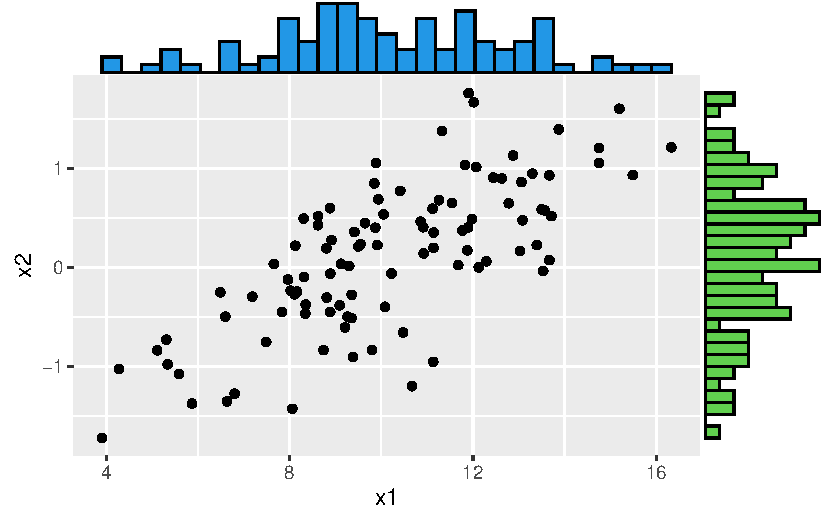
\includegraphics{LectureNotes/Lecture2_files/figure-pdf/unnamed-chunk-2-1.pdf}

\section{\texorpdfstring{{Building time series models from White
Noise}}{Building time series models from White Noise}}\label{building-time-series-models-from-white-noise}

\begin{longtable}[]{@{}
  >{\raggedright\arraybackslash}p{(\columnwidth - 4\tabcolsep) * \real{0.3333}}
  >{\raggedright\arraybackslash}p{(\columnwidth - 4\tabcolsep) * \real{0.3333}}
  >{\raggedright\arraybackslash}p{(\columnwidth - 4\tabcolsep) * \real{0.3333}}@{}}
\toprule\noalign{}
\begin{minipage}[b]{\linewidth}\raggedright
Model
\end{minipage} & \begin{minipage}[b]{\linewidth}\raggedright
Inputs
\end{minipage} & \begin{minipage}[b]{\linewidth}\raggedright
Output
\end{minipage} \\
\midrule\noalign{}
\endhead
\bottomrule\noalign{}
\endlastfoot
White noise & probability distribution, independence assumption,
\(\sigma_w^2\) & \\
Moving average with \(p\) points & \(w_1, w_2, \dots, w_n\) & \\
Autoregression of order \(p\) & \(w_1, w_2, \dots, w_n\) and
\(\phi = (\phi_1, \dots, \phi_p)\) & \\
Random walk with drift & \(w_1, w_2, \dots, w_n\) and \(\delta\) & \\
Signal plus noise & \(w_1, w_2, \dots, w_n\) and a function \(f(t)\)
& \\
\end{longtable}

Identify which of the inputs are random variables, pre-specified
constants, pre-specified functions, or parameters to be estimated.

\section{\texorpdfstring{{Building time series models from White
Noise}}{Building time series models from White Noise}}\label{building-time-series-models-from-white-noise-1}

\begin{longtable}[]{@{}
  >{\raggedright\arraybackslash}p{(\columnwidth - 4\tabcolsep) * \real{0.3333}}
  >{\raggedright\arraybackslash}p{(\columnwidth - 4\tabcolsep) * \real{0.3333}}
  >{\raggedright\arraybackslash}p{(\columnwidth - 4\tabcolsep) * \real{0.3333}}@{}}
\toprule\noalign{}
\begin{minipage}[b]{\linewidth}\raggedright
Model
\end{minipage} & \begin{minipage}[b]{\linewidth}\raggedright
Inputs
\end{minipage} & \begin{minipage}[b]{\linewidth}\raggedright
Output
\end{minipage} \\
\midrule\noalign{}
\endhead
\bottomrule\noalign{}
\endlastfoot
White noise & probability distribution, independence assumption,
\(\sigma_w^2\) & \(w_1, w_2, \dots, w_n\); for each \(t = 1, \dots, n\)
we have \(w_t \sim N(0, \sigma^2_w)\) \\
Moving average with \(p\) points & \(w_1, w_2, \dots, w_n\) &
\(v_t = \frac{1}{p}\sum_{i = 1}^{p} w_{t-(p-i)}\) \\
Autoregression of order \(p\) & \(w_1, w_2, \dots, w_n\) and
\(\phi = (\phi_1, \dots, \phi_p)\) &
\(x_t = \sum_{i = 1}^p \phi_ix_{t-i} + w_t\) \\
Random walk with drift & \(w_1, w_2, \dots, w_n\) and \(\delta\) &
\(x_t = \delta + x_{t-1} + w_t\) \\
Signal plus noise & \(w_1, w_2, \dots, w_n\) and a function \(f(t)\) &
\(x_t = f(t) + w_t\) \\
\end{longtable}

Identify which of the inputs are random variables, pre-specified
constants, pre-specified functions, or parameters to be estimated.

\section{Notation and Data}\label{notation-and-data}

Consider the general version of the autoregressive model of order 1:

\[
x_t = \phi_1x_{t-1} + \phi_2x_{t-2} + w_t
\]

If you had data representing this process, what would it look like in R?

\section{Notation and Data}\label{notation-and-data-1}

Suppose \(\phi_1 = 1.5\) and \(\phi_2 = -0.75\).

\begin{Shaded}
\begin{Highlighting}[]
\FunctionTok{set.seed}\NormalTok{(}\DecValTok{90210}\NormalTok{)}
\NormalTok{w }\OtherTok{=} \FunctionTok{rnorm}\NormalTok{(}\DecValTok{250} \SpecialCharTok{+} \DecValTok{50}\NormalTok{) }\CommentTok{\# 50 extra to avoid startup problems}
\NormalTok{x }\OtherTok{=} \FunctionTok{filter}\NormalTok{(w, }\AttributeTok{filter=}\FunctionTok{c}\NormalTok{(}\FloatTok{1.5}\NormalTok{,}\SpecialCharTok{{-}}\NormalTok{.}\DecValTok{75}\NormalTok{), }\AttributeTok{method=}\StringTok{"recursive"}\NormalTok{)[}\SpecialCharTok{{-}}\NormalTok{(}\DecValTok{1}\SpecialCharTok{:}\DecValTok{50}\NormalTok{)]}
\NormalTok{x}
\end{Highlighting}
\end{Shaded}

\begin{verbatim}
  [1] -0.635871231 -3.159366457 -3.336983558 -0.670017029  1.928041062
  [6]  6.262719337  8.811276769  6.994297589  6.964249838  4.172630149
 [11]  0.109387891 -2.838470465 -3.650839732 -5.293859716 -4.924149166
 [16] -3.496962661 -0.001206165  3.982335012  5.166059171  5.391303364
 [21]  4.598152813  2.726933281 -0.656314289 -2.634587218 -3.070392399
 [26] -2.447369835 -2.377035961 -3.272222376 -2.212579163 -1.609152064
 [31]  0.088151906  1.834292884  1.566977751  1.162326919  1.731270484
 [36]  0.452095019  0.751851590  2.197474589  2.037090911  2.053962776
 [41]  1.057859241  0.173798276 -1.559467228 -1.275347235 -1.934447794
 [46] -0.637721288  1.108281203  1.703590245  2.757116948  3.535041828
 [51]  2.785518718 -0.255025902 -3.601017151 -5.665073618 -5.320832378
 [56] -3.801870752 -1.843797185  0.540063136  1.577259338  2.719389114
 [61]  2.386440948  0.360417214  0.130240105  1.213682241  0.970840444
 [66]  1.672645132  1.169230978 -0.197824215 -0.552895930  0.483295378
 [71]  2.002207259  2.483139041  4.761206339  7.166338800  7.329547964
 [76]  5.238955522  1.955859515 -1.445155254 -3.624225029 -3.976740747
 [81] -2.522488940 -0.560280191  1.716462129  2.956985039  3.167747954
 [86]  2.655920142  2.503263867  0.243980727 -1.733850533  0.218414375
 [91]  1.212655465  1.188737220 -0.024525903  0.824315000 -0.929797989
 [96] -3.643408960 -4.872924684 -5.365789994 -4.379073769 -0.816292614
[101]  2.069716217  3.317790830  4.024356559  4.445225438  4.807260941
[106]  3.077726417  0.597309443 -1.889650709 -3.193428803 -4.189085934
[111] -5.056410971 -5.113692514 -1.701862879  0.197898712  1.872046685
[116]  2.519653174  1.995693810  1.375972346  2.342728546  1.412737664
[121] -1.604693814 -4.224595521 -6.808370201 -8.238970434 -7.267053979
[126] -5.073807901 -0.614874790  1.926334410  3.620792660  4.301297376
[131]  2.938794190  2.482699730  2.062144627  0.145550378 -2.263580334
[136] -3.515516041 -5.626740964 -5.675586843 -5.285219511 -3.877662550
[141] -2.843191932 -2.159754220 -1.134175851  0.621526810  2.144676177
[146]  1.301986893  1.090681772  0.483465932 -1.699760373 -0.907358670
[151] -1.964189610 -2.083464483 -2.401372850 -1.102177741  0.090984198
[156]  1.539763874  1.675986590  1.340872200 -0.451023892 -1.070116007
[161] -1.485934032  0.223487236  2.011408533  1.630095949  3.323091734
[166]  4.997983168  5.156394449  4.241727271  0.336603262 -1.668930450
[171] -3.056412007 -2.346607210  0.799083342  0.765047225  0.480923824
[176]  0.301524245  1.422952841  2.820001236  3.981388964  2.988835261
[181] -0.058956147 -2.066827932 -4.518505369 -5.447774381 -5.746818410
[186] -5.473607376 -3.515892394  0.432262861  4.283988479  6.685899229
[191]  6.379550991  5.781828167  5.127569880  2.228597185  1.512254758
[196]  1.407053783 -0.275040161 -2.623401872 -4.707758722 -6.845203817
[201] -8.189848947 -8.441072069 -5.100352049 -1.929194703 -0.289395357
[206]  2.511067946  4.007902754  2.638931037  0.953911823 -0.914044608
[211] -3.131803887 -4.574239309 -4.239263041 -1.278975512 -1.720543477
[216] -1.393708189 -0.978071153 -0.052109821 -0.479546542 -1.072444773
[221] -1.940146902 -2.221618511 -1.892476988 -0.145214604  1.941929437
[226]  2.662695670  1.548128421  1.266366609 -1.415637008 -2.255649300
[231] -2.492380384 -1.758574495 -0.272146596  1.472164787  1.788881267
[236]  0.946614002 -0.426152284  0.059796487 -2.263388225 -4.255693202
[241] -5.023127496 -5.240398677 -5.705131625 -3.494170488 -0.385992861
[246]  1.270003055  3.142585019  5.720389808  5.393790259  1.711581565
\end{verbatim}

\section{R example - Moving Average}\label{r-example---moving-average}

\begin{Shaded}
\begin{Highlighting}[]
\FunctionTok{set.seed}\NormalTok{(}\DecValTok{70}\NormalTok{)}

\CommentTok{\# generate white noise}
\NormalTok{w\_t }\OtherTok{\textless{}{-}} \FunctionTok{rnorm}\NormalTok{(}\DecValTok{10}\NormalTok{, }\DecValTok{0}\NormalTok{, }\DecValTok{1}\NormalTok{)}

\DocumentationTok{\#\# manually lag terms}
\NormalTok{w\_t1 }\OtherTok{\textless{}{-}} \FunctionTok{c}\NormalTok{(}\ConstantTok{NA}\NormalTok{, w\_t[}\DecValTok{1}\SpecialCharTok{:}\DecValTok{9}\NormalTok{])}
\NormalTok{w\_t2 }\OtherTok{\textless{}{-}} \FunctionTok{c}\NormalTok{(}\ConstantTok{NA}\NormalTok{, }\ConstantTok{NA}\NormalTok{, w\_t[}\DecValTok{1}\SpecialCharTok{:}\DecValTok{8}\NormalTok{])}

\DocumentationTok{\#\# manually compute MA(3)}
\NormalTok{v\_t }\OtherTok{\textless{}{-}}\NormalTok{ (w\_t }\SpecialCharTok{+}\NormalTok{ w\_t1 }\SpecialCharTok{+}\NormalTok{ w\_t2)}\SpecialCharTok{/}\DecValTok{3}

\DocumentationTok{\#\# compare the vectors}
\NormalTok{ma\_3 }\OtherTok{\textless{}{-}} \FunctionTok{cbind}\NormalTok{(v\_t, w\_t, w\_t1, w\_t2)}
\FunctionTok{round}\NormalTok{(ma\_3, }\DecValTok{3}\NormalTok{)}
\end{Highlighting}
\end{Shaded}

\begin{verbatim}
         v_t    w_t   w_t1   w_t2
 [1,]     NA -1.542     NA     NA
 [2,]     NA  0.347 -1.542     NA
 [3,] -0.032  1.099  0.347 -1.542
 [4,]  0.316 -0.499  1.099  0.347
 [5,] -0.112 -0.938 -0.499  1.099
 [6,] -0.523 -0.132 -0.938 -0.499
 [7,] -0.265  0.276 -0.132 -0.938
 [8,] -0.087 -0.405  0.276 -0.132
 [9,] -0.609 -1.696 -0.405  0.276
[10,] -0.569  0.394 -1.696 -0.405
\end{verbatim}

\begin{Shaded}
\begin{Highlighting}[]
\DocumentationTok{\#\# plot}
\CommentTok{\#par(mfrow = 2:1)}
\FunctionTok{plot}\NormalTok{(}\DecValTok{1}\SpecialCharTok{:}\DecValTok{10}\NormalTok{, w\_t, }\AttributeTok{type =} \StringTok{"b"}\NormalTok{, }\AttributeTok{lwd =} \DecValTok{2}\NormalTok{, }\AttributeTok{pch =} \DecValTok{16}\NormalTok{, }\AttributeTok{col =} \StringTok{"darkgrey"}\NormalTok{)}
\FunctionTok{points}\NormalTok{(}\DecValTok{1}\SpecialCharTok{:}\DecValTok{10}\NormalTok{, v\_t, }\AttributeTok{type =} \StringTok{"b"}\NormalTok{, }\AttributeTok{lwd =} \DecValTok{2}\NormalTok{, }\AttributeTok{pch =} \DecValTok{17}\NormalTok{, }\AttributeTok{col =} \StringTok{"blueviolet"}\NormalTok{)}
\end{Highlighting}
\end{Shaded}

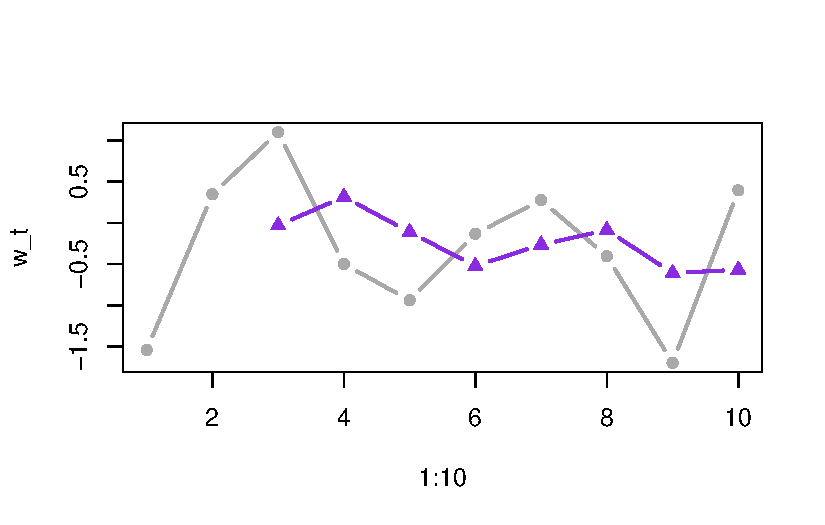
\includegraphics{LectureNotes/Lecture2_files/figure-pdf/unnamed-chunk-5-1.pdf}

\section{R example - Moving Average}\label{r-example---moving-average-1}

\begin{Shaded}
\begin{Highlighting}[]
\CommentTok{\# generate white noise}
\NormalTok{n }\OtherTok{=} \DecValTok{50}
\NormalTok{w\_t }\OtherTok{\textless{}{-}} \FunctionTok{rnorm}\NormalTok{(n, }\DecValTok{0}\NormalTok{, }\DecValTok{1}\NormalTok{)}

\DocumentationTok{\#\# manually lag terms}
\NormalTok{w\_t1 }\OtherTok{\textless{}{-}} \FunctionTok{c}\NormalTok{(}\ConstantTok{NA}\NormalTok{, w\_t[}\DecValTok{1}\SpecialCharTok{:}\NormalTok{(n}\DecValTok{{-}1}\NormalTok{)])}
\NormalTok{w\_t2 }\OtherTok{\textless{}{-}} \FunctionTok{c}\NormalTok{(}\ConstantTok{NA}\NormalTok{, }\ConstantTok{NA}\NormalTok{, w\_t[}\DecValTok{1}\SpecialCharTok{:}\NormalTok{(n}\DecValTok{{-}2}\NormalTok{)])}

\DocumentationTok{\#\# manually compute MA(3)}
\NormalTok{v\_t }\OtherTok{\textless{}{-}}\NormalTok{ (w\_t }\SpecialCharTok{+}\NormalTok{ w\_t1 }\SpecialCharTok{+}\NormalTok{ w\_t2)}\SpecialCharTok{/}\DecValTok{3}

\DocumentationTok{\#\# compare the vectors}
\NormalTok{ma\_3 }\OtherTok{\textless{}{-}} \FunctionTok{cbind}\NormalTok{(v\_t, w\_t, w\_t1, w\_t2)}
\FunctionTok{round}\NormalTok{(ma\_3, }\DecValTok{3}\NormalTok{)}
\end{Highlighting}
\end{Shaded}

\begin{verbatim}
         v_t    w_t   w_t1   w_t2
 [1,]     NA -0.834     NA     NA
 [2,]     NA  0.799 -0.834     NA
 [3,]  0.043  0.163  0.799 -0.834
 [4,]  0.752  1.292  0.163  0.799
 [5,]  0.491  0.018  1.292  0.163
 [6,]  0.435 -0.006  0.018  1.292
 [7,]  0.163  0.476 -0.006  0.018
 [8,]  0.652  1.486  0.476 -0.006
 [9,]  0.592 -0.186  1.486  0.476
[10,]  0.778  1.034 -0.186  1.486
[11,] -0.016 -0.896  1.034 -0.186
[12,]  0.006 -0.121 -0.896  1.034
[13,] -0.475 -0.408 -0.121 -0.896
[14,] -0.170  0.019 -0.408 -0.121
[15,] -0.164 -0.102  0.019 -0.408
[16,] -0.727 -2.098 -0.102  0.019
[17,] -0.798 -0.195 -2.098 -0.102
[18,] -0.996 -0.697 -0.195 -2.098
[19,] -0.145  0.457 -0.697 -0.195
[20,]  0.225  0.914  0.457 -0.697
[21,]  0.895  1.314  0.914  0.457
[22,]  0.410 -0.998  1.314  0.914
[23,] -0.048 -0.459 -0.998  1.314
[24,] -0.546 -0.181 -0.459 -0.998
[25,] -0.252 -0.116 -0.181 -0.459
[26,] -0.105 -0.017 -0.116 -0.181
[27,] -0.227 -0.547 -0.017 -0.116
[28,] -0.052  0.408 -0.547 -0.017
[29,] -0.231 -0.555  0.408 -0.547
[30,] -0.168 -0.356 -0.555  0.408
[31,] -0.328 -0.074 -0.356 -0.555
[32,] -0.608 -1.393 -0.074 -0.356
[33,] -0.604 -0.345 -1.393 -0.074
[34,] -1.214 -1.904 -0.345 -1.393
[35,] -0.917 -0.503 -1.904 -0.345
[36,] -0.564  0.715 -0.503 -1.904
[37,]  0.173  0.306  0.715 -0.503
[38,]  0.572  0.694  0.306  0.715
[39,]  0.361  0.083  0.694  0.306
[40,]  0.281  0.065  0.083  0.694
[41,]  0.308  0.776  0.065  0.083
[42,]  0.413  0.397  0.776  0.065
[43,]  0.162 -0.686  0.397  0.776
[44,] -0.371 -0.824 -0.686  0.397
[45,] -0.745 -0.725 -0.824 -0.686
[46,]  0.026  1.627 -0.725 -0.824
[47,]  0.733  1.298  1.627 -0.725
[48,]  0.424 -1.653  1.298  1.627
[49,] -0.927 -2.427 -1.653  1.298
[50,] -1.123  0.710 -2.427 -1.653
\end{verbatim}

\begin{Shaded}
\begin{Highlighting}[]
\DocumentationTok{\#\# plot}
\CommentTok{\#par(mfrow = 2:1)}
\FunctionTok{plot}\NormalTok{(}\DecValTok{1}\SpecialCharTok{:}\NormalTok{n, w\_t, }\AttributeTok{type =} \StringTok{"b"}\NormalTok{, }\AttributeTok{lwd =} \DecValTok{2}\NormalTok{, }\AttributeTok{pch =} \DecValTok{16}\NormalTok{, }\AttributeTok{col =} \StringTok{"darkgrey"}\NormalTok{)}
\FunctionTok{points}\NormalTok{(}\DecValTok{1}\SpecialCharTok{:}\NormalTok{n, v\_t, }\AttributeTok{type =} \StringTok{"b"}\NormalTok{, }\AttributeTok{lwd =} \DecValTok{2}\NormalTok{, }\AttributeTok{pch =} \DecValTok{17}\NormalTok{, }\AttributeTok{col =} \StringTok{"blueviolet"}\NormalTok{)}
\end{Highlighting}
\end{Shaded}

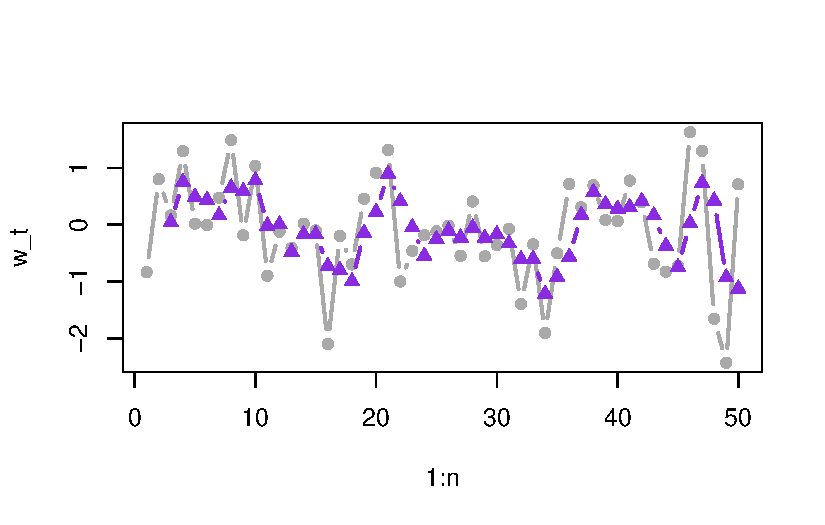
\includegraphics{LectureNotes/Lecture2_files/figure-pdf/unnamed-chunk-7-1.pdf}

\chapter{Chapter 2: Correlation and Stationary Time
Series}\label{chapter-2-correlation-and-stationary-time-series}

\section{Motivation}\label{motivation}

How do we summarize characteristics of a distribution?

\begin{Shaded}
\begin{Highlighting}[]
\FunctionTok{set.seed}\NormalTok{(}\DecValTok{2024}\NormalTok{)}
\NormalTok{x }\OtherTok{\textless{}{-}} \FunctionTok{rnorm}\NormalTok{(}\DecValTok{1000}\NormalTok{, }\DecValTok{10}\NormalTok{, }\DecValTok{1}\NormalTok{)}
\NormalTok{y }\OtherTok{\textless{}{-}} \FunctionTok{rnorm}\NormalTok{(}\DecValTok{1000}\NormalTok{, }\DecValTok{8}\NormalTok{, .}\DecValTok{75}\NormalTok{)}
\NormalTok{z }\OtherTok{\textless{}{-}} \FunctionTok{c}\NormalTok{(x,y)}
\FunctionTok{hist}\NormalTok{(z)}
\end{Highlighting}
\end{Shaded}

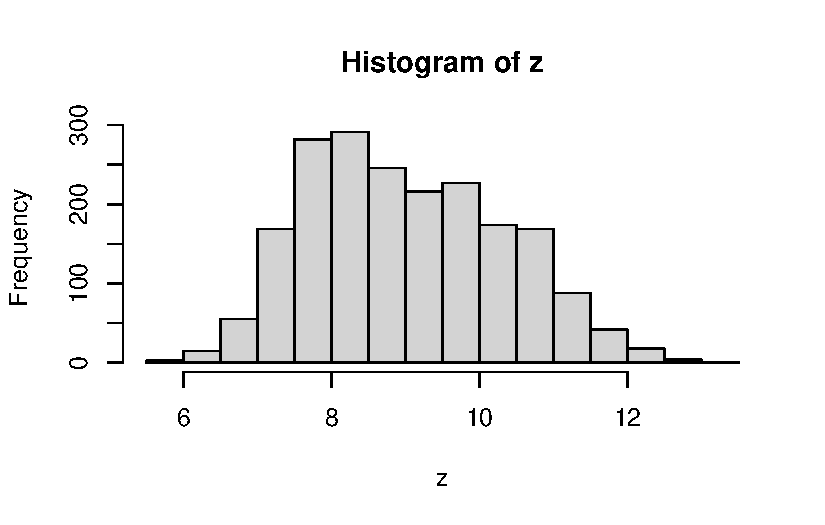
\includegraphics{LectureNotes/Lecture2_files/figure-pdf/unnamed-chunk-8-1.pdf}

\section{Motivation}\label{motivation-1}

How do we summarize characteristics of a distribution?

\begin{itemize}
\item
  mean
\item
  variance(standard deviation)
\end{itemize}

\begin{Shaded}
\begin{Highlighting}[]
\FunctionTok{hist}\NormalTok{(z)}
\FunctionTok{abline}\NormalTok{(}\AttributeTok{v =} \FunctionTok{mean}\NormalTok{(z), }\AttributeTok{col =} \StringTok{"red"}\NormalTok{, }\AttributeTok{lwd =} \DecValTok{2}\NormalTok{)}
\FunctionTok{abline}\NormalTok{(}\AttributeTok{v =} \FunctionTok{mean}\NormalTok{(z) }\SpecialCharTok{+} \FunctionTok{sd}\NormalTok{(z), }\AttributeTok{col =} \StringTok{"blue"}\NormalTok{, }\AttributeTok{lty =} \DecValTok{2}\NormalTok{, }\AttributeTok{lwd =} \DecValTok{2}\NormalTok{)}
\FunctionTok{abline}\NormalTok{(}\AttributeTok{v =} \FunctionTok{mean}\NormalTok{(z) }\SpecialCharTok{{-}} \FunctionTok{sd}\NormalTok{(z), }\AttributeTok{col =} \StringTok{"blue"}\NormalTok{, }\AttributeTok{lty =} \DecValTok{2}\NormalTok{, }\AttributeTok{lwd =} \DecValTok{2}\NormalTok{)}
\FunctionTok{text}\NormalTok{(}\AttributeTok{x =} \DecValTok{11}\NormalTok{, }\AttributeTok{y =} \DecValTok{225}\NormalTok{, }
     \AttributeTok{labels =} \FunctionTok{paste}\NormalTok{(}\StringTok{"mean = "}\NormalTok{, }\FunctionTok{round}\NormalTok{(}\FunctionTok{mean}\NormalTok{(z),}\DecValTok{2}\NormalTok{), }
                    \StringTok{"}\SpecialCharTok{\textbackslash{}n}\StringTok{ sd = "}\NormalTok{, }\FunctionTok{round}\NormalTok{(}\FunctionTok{sd}\NormalTok{(z),}\DecValTok{2}\NormalTok{)))}
\end{Highlighting}
\end{Shaded}

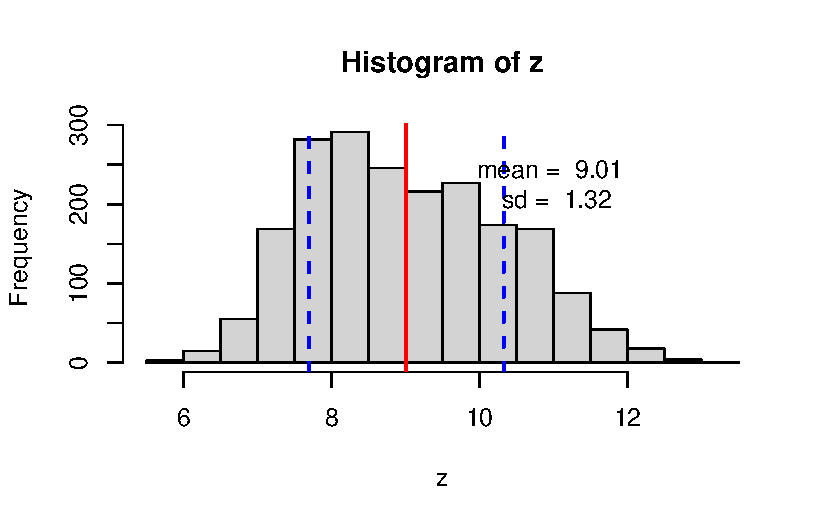
\includegraphics{LectureNotes/Lecture2_files/figure-pdf/unnamed-chunk-9-1.pdf}

\section{How do we summarize the characteristics of a distribution that
changes over
time?}\label{how-do-we-summarize-the-characteristics-of-a-distribution-that-changes-over-time}

\begin{itemize}
\item
  mean function (of time)
\item
  (auto)(co)variance function (of time)
\end{itemize}

\chapter{Mean function}\label{mean-function}

\section{Mean Function}\label{mean-function-1}

The mean function of a time series \(x_t\) is defined as:

\[
\mu_{xt} = \E(x_t) = \int_{-\infty}^\infty x_tf(x_t)dx_t,
\]

where \(\E\) is the expected value operator, shown here for the case of
a continuous \(x_t\).\\

So, for example, if \(x_t\) is normally distributed then \(f\) here
would be the normal probability density function (p.d.f.).

\section{Visual examples}\label{visual-examples}

\begin{Shaded}
\begin{Highlighting}[]
\FunctionTok{library}\NormalTok{(astsa)}
\FunctionTok{set.seed}\NormalTok{(}\DecValTok{314159265}\NormalTok{) }\CommentTok{\# so you can reproduce the results}
\NormalTok{w  }\OtherTok{=} \FunctionTok{rnorm}\NormalTok{(}\DecValTok{200}\NormalTok{)  }\DocumentationTok{\#\# Gaussian white noise}
\NormalTok{x  }\OtherTok{=} \FunctionTok{cumsum}\NormalTok{(w)}
\NormalTok{wd }\OtherTok{=}\NormalTok{ w }\SpecialCharTok{+}\NormalTok{.}\DecValTok{3} 
\NormalTok{xd }\OtherTok{=} \FunctionTok{cumsum}\NormalTok{(wd)}
\FunctionTok{tsplot}\NormalTok{(xd, }\AttributeTok{ylim=}\FunctionTok{c}\NormalTok{(}\SpecialCharTok{{-}}\DecValTok{2}\NormalTok{,}\DecValTok{80}\NormalTok{), }\AttributeTok{main=}\StringTok{"random walk"}\NormalTok{, }\AttributeTok{ylab=}\StringTok{""}\NormalTok{, }\AttributeTok{col=}\DecValTok{4}\NormalTok{)}
 \FunctionTok{clip}\NormalTok{(}\DecValTok{0}\NormalTok{, }\DecValTok{200}\NormalTok{, }\DecValTok{0}\NormalTok{, }\DecValTok{80}\NormalTok{)}
 \FunctionTok{abline}\NormalTok{(}\AttributeTok{a=}\DecValTok{0}\NormalTok{, }\AttributeTok{b=}\NormalTok{.}\DecValTok{3}\NormalTok{, }\AttributeTok{lty=}\DecValTok{2}\NormalTok{, }\AttributeTok{col=}\DecValTok{4}\NormalTok{) }\CommentTok{\# drift}
\FunctionTok{lines}\NormalTok{(x, }\AttributeTok{col=}\DecValTok{6}\NormalTok{)}
 \FunctionTok{clip}\NormalTok{(}\DecValTok{0}\NormalTok{, }\DecValTok{200}\NormalTok{, }\DecValTok{0}\NormalTok{, }\DecValTok{80}\NormalTok{)}
 \FunctionTok{abline}\NormalTok{(}\AttributeTok{h=}\DecValTok{0}\NormalTok{, }\AttributeTok{col=}\DecValTok{6}\NormalTok{, }\AttributeTok{lty=}\DecValTok{2}\NormalTok{)}
\end{Highlighting}
\end{Shaded}

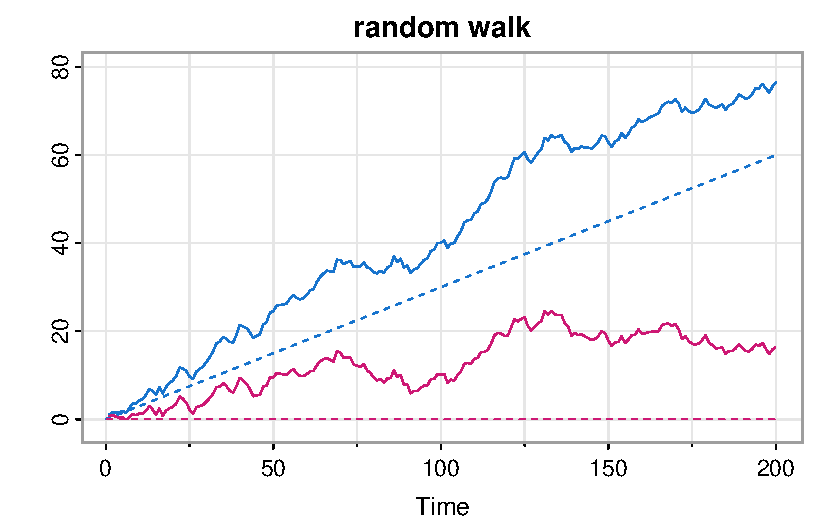
\includegraphics{LectureNotes/Lecture2_files/figure-pdf/unnamed-chunk-10-1.pdf}

\section{Visual examples}\label{visual-examples-1}

\begin{Shaded}
\begin{Highlighting}[]
\CommentTok{\# cs = 2*cos(2*pi*(1:500)/50 + .6*pi)    \# as in the text}
\NormalTok{cs }\OtherTok{=} \DecValTok{2}\SpecialCharTok{*}\FunctionTok{cos}\NormalTok{(}\DecValTok{2}\SpecialCharTok{*}\NormalTok{pi}\SpecialCharTok{*}\NormalTok{(}\DecValTok{1}\SpecialCharTok{:}\DecValTok{500}\SpecialCharTok{+}\DecValTok{15}\NormalTok{)}\SpecialCharTok{/}\DecValTok{50}\NormalTok{)           }\CommentTok{\# same thing }
\NormalTok{w  }\OtherTok{=} \FunctionTok{rnorm}\NormalTok{(}\DecValTok{500}\NormalTok{,}\DecValTok{0}\NormalTok{,}\DecValTok{1}\NormalTok{)}
\FunctionTok{par}\NormalTok{(}\AttributeTok{mfrow=}\FunctionTok{c}\NormalTok{(}\DecValTok{3}\NormalTok{,}\DecValTok{1}\NormalTok{))   }
\FunctionTok{tsplot}\NormalTok{(cs }\SpecialCharTok{+}\NormalTok{ w, }\AttributeTok{ylab=}\StringTok{""}\NormalTok{, }\AttributeTok{main =} \FunctionTok{expression}\NormalTok{(x[t]}\SpecialCharTok{==}\DecValTok{2}\SpecialCharTok{*}\FunctionTok{cos}\NormalTok{(}\DecValTok{2}\SpecialCharTok{*}\NormalTok{pi}\SpecialCharTok{*}\NormalTok{t}\SpecialCharTok{/}\DecValTok{50}\FloatTok{+.6}\SpecialCharTok{*}\NormalTok{pi)}\SpecialCharTok{+}\FunctionTok{N}\NormalTok{(}\DecValTok{0}\NormalTok{,}\DecValTok{1}\NormalTok{)))}
\FunctionTok{points}\NormalTok{(cs, }\AttributeTok{ylab=}\StringTok{""}\NormalTok{, }\AttributeTok{main =} \FunctionTok{expression}\NormalTok{(x[t]}\SpecialCharTok{==}\DecValTok{2}\SpecialCharTok{*}\FunctionTok{cos}\NormalTok{(}\DecValTok{2}\SpecialCharTok{*}\NormalTok{pi}\SpecialCharTok{*}\NormalTok{t}\SpecialCharTok{/}\DecValTok{50}\FloatTok{+.6}\SpecialCharTok{*}\NormalTok{pi)), }\AttributeTok{type =} \StringTok{"l"}\NormalTok{, }\AttributeTok{col =} \StringTok{"blueviolet"}\NormalTok{, }\AttributeTok{lwd =} \DecValTok{2}\NormalTok{)}
\FunctionTok{tsplot}\NormalTok{(cs }\SpecialCharTok{+} \DecValTok{5}\SpecialCharTok{*}\NormalTok{w, }\AttributeTok{ylab=}\StringTok{""}\NormalTok{, }\AttributeTok{main =} \FunctionTok{expression}\NormalTok{(x[t]}\SpecialCharTok{==}\DecValTok{2}\SpecialCharTok{*}\FunctionTok{cos}\NormalTok{(}\DecValTok{2}\SpecialCharTok{*}\NormalTok{pi}\SpecialCharTok{*}\NormalTok{t}\SpecialCharTok{/}\DecValTok{50}\FloatTok{+.6}\SpecialCharTok{*}\NormalTok{pi)}\SpecialCharTok{+}\FunctionTok{N}\NormalTok{(}\DecValTok{0}\NormalTok{,}\DecValTok{25}\NormalTok{)))}
\FunctionTok{points}\NormalTok{(cs, }\AttributeTok{ylab=}\StringTok{""}\NormalTok{, }\AttributeTok{main =} \FunctionTok{expression}\NormalTok{(x[t]}\SpecialCharTok{==}\DecValTok{2}\SpecialCharTok{*}\FunctionTok{cos}\NormalTok{(}\DecValTok{2}\SpecialCharTok{*}\NormalTok{pi}\SpecialCharTok{*}\NormalTok{t}\SpecialCharTok{/}\DecValTok{50}\FloatTok{+.6}\SpecialCharTok{*}\NormalTok{pi)), }\AttributeTok{type =} \StringTok{"l"}\NormalTok{, }\AttributeTok{col =} \StringTok{"blueviolet"}\NormalTok{, }\AttributeTok{lwd =} \DecValTok{2}\NormalTok{)}
\end{Highlighting}
\end{Shaded}

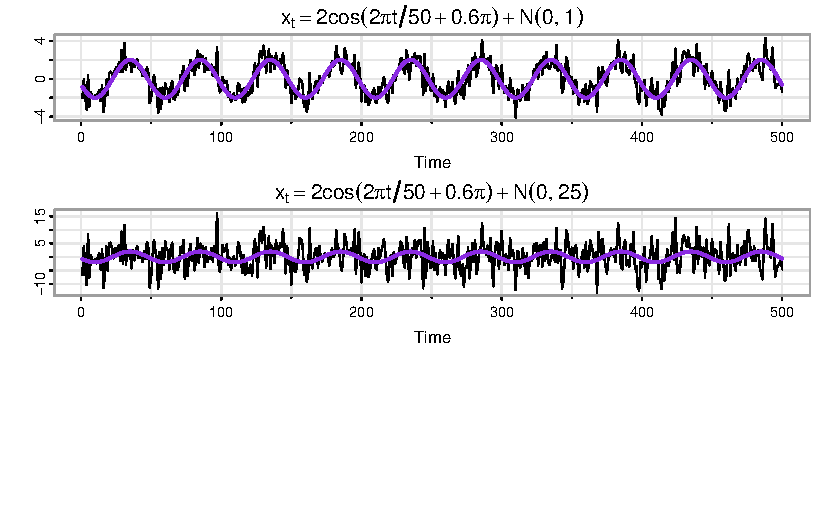
\includegraphics{LectureNotes/Lecture2_files/figure-pdf/unnamed-chunk-11-1.pdf}

\section{Notating the mean function}\label{notating-the-mean-function}

\emph{``When no confusion exists about which time series we are
referring to, we will drop a subscript and write} \(\mu_{xt}\) \emph{as}
\(\mu_t\)\emph{.''}

Confusion might exist if we have two time series e.g.~if

\begin{itemize}
\item
  \(x_t\) is the SOI for a given month and
\item
  \(y_t\) is the estimated new fish for a given month
\end{itemize}

we would have two mean functions, \(\mu_{yt}\) and \(\mu_{xt}\).

\section{Example 2.2 Mean Function of a Moving Average
Series}\label{example-2.2-mean-function-of-a-moving-average-series}

Let \(w_t\) denote a white noise series.

\begin{itemize}
\tightlist
\item
  What is \(\mu_{wt} = \E(w_t)\) ?
\end{itemize}

Let \(v_t = \frac{1}{3}(w_{t-1} + w_{t} + w_{t+1})\) .

\begin{itemize}
\tightlist
\item
  What is \(\mu_{vt} = \E(v_t)\)?
\end{itemize}

(why not just write \(\mu_t\) on this slide?)

\section{Example 2.3 Mean Function of a Random Walk with
drift}\label{example-2.3-mean-function-of-a-random-walk-with-drift}

Look, it's our friend the random walk with drift (maybe):

\[
x_t = \delta t + \sum_{j = 1}^t w_j
\]

What is the mean function of \(x_t\)?

\section{Break}\label{break}

\begin{itemize}
\tightlist
\item
  I saw several turkeys this morning
\item
  I saw someone almost die on a skateboard
\end{itemize}

\chapter{Autocovariance}\label{autocovariance}

\section{Does the mean function tell us anything about the
(in)dependence of the time
series?}\label{does-the-mean-function-tell-us-anything-about-the-independence-of-the-time-series}

No (expected value is such a friendly operator!)

\section{Review: Variance and
Covariance}\label{review-variance-and-covariance}

If \(X\) is a random variable and then \(\E(X) = \mu\),

\[
Var(X) = \E((X-\mu)^2)
\] If we have two random variables \(X_\alpha\) and \(X_\beta\), the
covariance between these is \[
Cov(X_\alpha, X_\beta) = \E[(X_\alpha - \mu_\alpha)(X_\beta - \mu_\beta)]
\] - remember correlation (scaled covariance)??

\section{Autocovariance function}\label{autocovariance-function}

The autocovariance function is defined as the second moment product \[
\gamma_x(s, t) = cov(x_s, x_t) = \E[(x_s - \mu_s)(x_t - \mu_t)]
\] for all \(s\) and \(t\).

\begin{itemize}
\tightlist
\item
  When no confusion exists, we will drop the \(x\) as with the mean
  function i.e.~\(\gamma(s, t)\) instead of \(\gamma_x(s, t)\)
\item
  How can we write \(var(x_t)\) in terms of \(\gamma\)? \[
  \gamma_x(t,t) = \E[(x_t - \mu_t)^2] = var(x_t) 
  \]
\end{itemize}

\section{Example 2.6 Autocovariance of White
Noise}\label{example-2.6-autocovariance-of-white-noise}

\(w_t\) ⬅️ white noise series

\(\gamma_w(s, t) = cov(w_s, w_t) = \text{ }?\)

\section{Example 2.6 Autocovariance of White
Noise}\label{example-2.6-autocovariance-of-white-noise-1}

\(w_t\) ⬅️ white noise series

\(\gamma_w(s, t) = cov(w_s, w_t) =  \begin{cases} \sigma^2_w & \text{ if } s = t\\ 0 & \text{ if } s \ne t \end{cases}\)

\section{Example 2.8 Autocovariance of a Moving
Average}\label{example-2.8-autocovariance-of-a-moving-average}

Consider three point moving average
\(v_t = \frac{1}{3}(w_{t-1} + w_t + w_{t+1})\)

\(\gamma_v(s, t) = cov(v_s, v_t) =  \begin{cases}a & \text{ if } s = t\\ b & \text{ if } \vert s-t \vert = 1 \\c& \text{ if } \vert s-t \vert =2 \\ d & \text{ if } \vert s - t\vert > 2\end{cases}\)

\begin{itemize}
\tightlist
\item
  Which one of \(a, b, c, d\) is 0
\item
  Are \(a, b, c\) the same? If not, which is largest?
\end{itemize}

\section{Example 2.8 Autocovariance of a Moving
Average}\label{example-2.8-autocovariance-of-a-moving-average-1}

Consider three point moving average
\(v_t = \frac{1}{3}(w_{t-1} + w_t + w_{t+1})\)

\(\gamma_v(s, t) = cov(v_s, v_t) =  \begin{cases}\frac{3}{9}\sigma^2_w & \text{ if } s = t\\ \frac{2}{9}\sigma^2_w & \text{ if } \vert s-t \vert = 1 \\\frac{1}{9}\sigma^2_w & \text{ if } \vert s-t \vert =2 \\0 & \text{ if } \vert s - t\vert > 2\end{cases}\)

Does this equation make intuitive sense?

\section{Example 2.9 Autocovariance of a Random
Walk}\label{example-2.9-autocovariance-of-a-random-walk}

\(x_t = \sum_{j = 1}^t w_j\)

\[
\gamma_x(s, t) = cov(x_s, x_t) = cov\left ( \sum_{j=1}^s w_j, \sum_{k = 1}^t w_k\right ) = \min\{s,t\}\sigma^2_w
\] If you waaaaant, property 2.7 and figuring out what \(\E(w_jw_k)\) is
for \(j \ne k\)

\chapter{In-class R problems}\label{in-class-r-problems}

\section{R example - Moving Average}\label{r-example---moving-average-2}

\begin{Shaded}
\begin{Highlighting}[]
\CommentTok{\# generate white noise}
\NormalTok{n }\OtherTok{=} \DecValTok{50}
\NormalTok{w\_t }\OtherTok{\textless{}{-}} \FunctionTok{rnorm}\NormalTok{(n, }\DecValTok{0}\NormalTok{, }\DecValTok{1}\NormalTok{)}

\DocumentationTok{\#\# manually lag terms}
\NormalTok{w\_t1 }\OtherTok{\textless{}{-}} \FunctionTok{c}\NormalTok{(}\ConstantTok{NA}\NormalTok{, w\_t[}\DecValTok{1}\SpecialCharTok{:}\NormalTok{(n}\DecValTok{{-}1}\NormalTok{)])}
\NormalTok{w\_t2 }\OtherTok{\textless{}{-}} \FunctionTok{c}\NormalTok{(}\ConstantTok{NA}\NormalTok{, }\ConstantTok{NA}\NormalTok{, w\_t[}\DecValTok{1}\SpecialCharTok{:}\NormalTok{(n}\DecValTok{{-}2}\NormalTok{)])}

\DocumentationTok{\#\# manually compute MA(3)}
\NormalTok{v\_t }\OtherTok{\textless{}{-}}\NormalTok{ ?}

\DocumentationTok{\#\# compare the vectors}
\NormalTok{ma\_3 }\OtherTok{\textless{}{-}} \FunctionTok{cbind}\NormalTok{(v\_t, w\_t, w\_t1, w\_t2, w\_t3)}
\FunctionTok{round}\NormalTok{(ma\_3, }\DecValTok{3}\NormalTok{)}

\DocumentationTok{\#\# also compute MA(3) using stats::filter}
\NormalTok{v\_t\_alt }\OtherTok{\textless{}{-}}\NormalTok{ ?}
  
\DocumentationTok{\#\# plot both}
\end{Highlighting}
\end{Shaded}

\section{R example - Moving Average}\label{r-example---moving-average-3}

\begin{Shaded}
\begin{Highlighting}[]
\CommentTok{\# generate white noise}
\NormalTok{n }\OtherTok{=} \DecValTok{50}
\NormalTok{w\_t }\OtherTok{\textless{}{-}} \FunctionTok{rnorm}\NormalTok{(n, }\DecValTok{0}\NormalTok{, }\DecValTok{1}\NormalTok{)}

\DocumentationTok{\#\# manually lag terms}
\NormalTok{w\_t1 }\OtherTok{\textless{}{-}} \FunctionTok{c}\NormalTok{(}\ConstantTok{NA}\NormalTok{, w\_t[}\DecValTok{1}\SpecialCharTok{:}\NormalTok{(n}\DecValTok{{-}1}\NormalTok{)])}
\NormalTok{w\_t2 }\OtherTok{\textless{}{-}} \FunctionTok{c}\NormalTok{(}\ConstantTok{NA}\NormalTok{, }\ConstantTok{NA}\NormalTok{, w\_t[}\DecValTok{1}\SpecialCharTok{:}\NormalTok{(n}\DecValTok{{-}2}\NormalTok{)])}
\NormalTok{w\_t3 }\OtherTok{\textless{}{-}} \FunctionTok{c}\NormalTok{(}\ConstantTok{NA}\NormalTok{, }\ConstantTok{NA}\NormalTok{, }\ConstantTok{NA}\NormalTok{, w\_t[}\DecValTok{1}\SpecialCharTok{:}\NormalTok{(n}\DecValTok{{-}3}\NormalTok{)])}
\DocumentationTok{\#\# manually compute MA(3)}
\NormalTok{v\_t }\OtherTok{\textless{}{-}}\NormalTok{ (w\_t }\SpecialCharTok{+}\NormalTok{ w\_t1 }\SpecialCharTok{+}\NormalTok{ w\_t2 }\SpecialCharTok{+}\NormalTok{ w\_t3)}\SpecialCharTok{/}\DecValTok{4}

\DocumentationTok{\#\# compare the vectors}
\NormalTok{ma\_3 }\OtherTok{\textless{}{-}} \FunctionTok{cbind}\NormalTok{(v\_t, w\_t, w\_t1, w\_t2, w\_t3)}
\FunctionTok{round}\NormalTok{(ma\_3, }\DecValTok{3}\NormalTok{)}
\end{Highlighting}
\end{Shaded}

\begin{verbatim}
         v_t    w_t   w_t1   w_t2   w_t3
 [1,]     NA  1.063     NA     NA     NA
 [2,]     NA  0.150  1.063     NA     NA
 [3,]     NA -1.161  0.150  1.063     NA
 [4,] -0.227 -0.958 -1.161  0.150  1.063
 [5,] -0.619 -0.507 -0.958 -1.161  0.150
 [6,] -0.807 -0.600 -0.507 -0.958 -1.161
 [7,] -0.913 -1.587 -0.600 -0.507 -0.958
 [8,] -0.710 -0.144 -1.587 -0.600 -0.507
 [9,] -0.790 -0.827 -0.144 -1.587 -0.600
[10,] -0.460  0.717 -0.827 -0.144 -1.587
[11,]  0.041  0.419  0.717 -0.827 -0.144
[12,]  0.198  0.483  0.419  0.717 -0.827
[13,]  0.463  0.235  0.483  0.419  0.717
[14,]  0.128 -0.624  0.235  0.483  0.419
[15,] -0.186 -0.837 -0.624  0.235  0.483
[16,]  0.053  1.438 -0.837 -0.624  0.235
[17,]  0.271  1.107  1.438 -0.837 -0.624
[18,]  0.512  0.342  1.107  1.438 -0.837
[19,]  0.468 -1.014  0.342  1.107  1.438
[20,]  0.577  1.871 -1.014  0.342  1.107
[21,]  0.100 -0.802  1.871 -1.014  0.342
[22,] -0.041 -0.221 -0.802  1.871 -1.014
[23,]  0.402  0.758 -0.221 -0.802  1.871
[24,]  0.390  1.823  0.758 -0.221 -0.802
[25,]  0.661  0.282  1.823  0.758 -0.221
[26,]  0.755  0.157  0.282  1.823  0.758
[27,]  0.805  0.956  0.157  0.282  1.823
[28,]  0.850  2.003  0.956  0.157  0.282
[29,]  0.892  0.453  2.003  0.956  0.157
[30,]  0.928  0.300  0.453  2.003  0.956
[31,]  0.822  0.531  0.300  0.453  2.003
[32,]  0.790  1.877  0.531  0.300  0.453
[33,]  0.551 -0.503  1.877  0.531  0.300
[34,]  0.239 -0.950 -0.503  1.877  0.531
[35,]  0.383  1.110 -0.950 -0.503  1.877
[36,] -0.425 -1.357  1.110 -0.950 -0.503
[37,] -0.033  1.063 -1.357  1.110 -0.950
[38,] -0.151 -1.422  1.063 -1.357  1.110
[39,] -0.310  0.475 -1.422  1.063 -1.357
[40,] -0.133 -0.647  0.475 -1.422  1.063
[41,] -0.338  0.242 -0.647  0.475 -1.422
[42,] -0.002 -0.077  0.242 -0.647  0.475
[43,] -0.160 -0.159 -0.077  0.242 -0.647
[44,] -0.031 -0.129 -0.159 -0.077  0.242
[45,] -0.437 -1.383 -0.129 -0.159 -0.077
[46,]  0.237  2.620 -1.383 -0.129 -0.159
[47,] -0.023 -1.201  2.620 -1.383 -0.129
[48,]  0.182  0.690 -1.201  2.620 -1.383
[49,]  0.455 -0.290  0.690 -1.201  2.620
[50,]  0.288  1.954 -0.290  0.690 -1.201
\end{verbatim}

\begin{Shaded}
\begin{Highlighting}[]
\DocumentationTok{\#\# also compute using stats::filter}
\NormalTok{v\_t\_alt }\OtherTok{\textless{}{-}}\NormalTok{ stats}\SpecialCharTok{::}\FunctionTok{filter}\NormalTok{(w\_t, }\AttributeTok{sides =} \DecValTok{2}\NormalTok{, }\AttributeTok{filter =} \FunctionTok{rep}\NormalTok{(}\FloatTok{0.25}\NormalTok{, }\AttributeTok{times =} \DecValTok{4}\NormalTok{))}
\end{Highlighting}
\end{Shaded}

\begin{Shaded}
\begin{Highlighting}[]
\DocumentationTok{\#\# plot}
\CommentTok{\#par(mfrow = 2:1)}
\FunctionTok{plot}\NormalTok{(}\DecValTok{1}\SpecialCharTok{:}\NormalTok{n, w\_t, }\AttributeTok{type =} \StringTok{"b"}\NormalTok{, }\AttributeTok{lwd =} \DecValTok{2}\NormalTok{, }\AttributeTok{pch =} \DecValTok{16}\NormalTok{, }\AttributeTok{col =} \StringTok{"darkgrey"}\NormalTok{)}
\FunctionTok{points}\NormalTok{(}\DecValTok{1}\SpecialCharTok{:}\NormalTok{n, v\_t, }\AttributeTok{type =} \StringTok{"b"}\NormalTok{, }\AttributeTok{lwd =} \DecValTok{2}\NormalTok{, }\AttributeTok{pch =} \DecValTok{17}\NormalTok{, }\AttributeTok{col =} \StringTok{"blueviolet"}\NormalTok{)}
\end{Highlighting}
\end{Shaded}

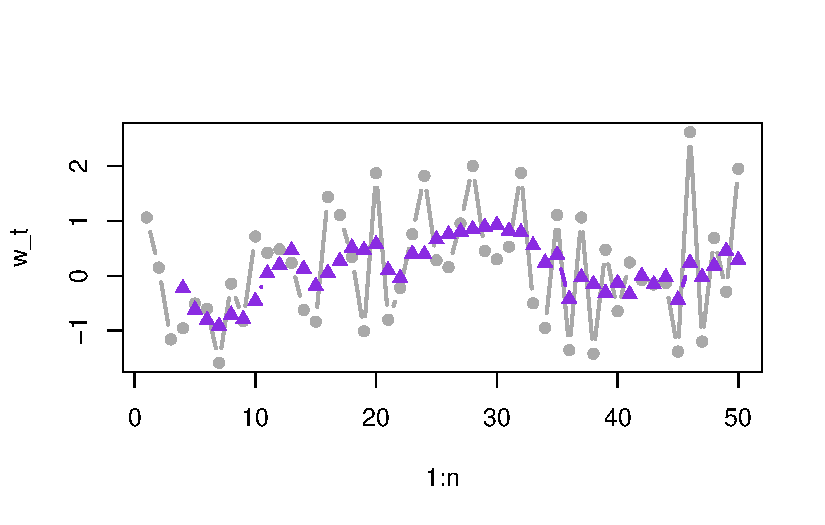
\includegraphics{LectureNotes/Lecture2_files/figure-pdf/unnamed-chunk-14-1.pdf}

\begin{Shaded}
\begin{Highlighting}[]
\FunctionTok{plot}\NormalTok{(}\DecValTok{1}\SpecialCharTok{:}\NormalTok{n, w\_t, }\AttributeTok{type =} \StringTok{"b"}\NormalTok{, }\AttributeTok{lwd =} \DecValTok{2}\NormalTok{, }\AttributeTok{pch =} \DecValTok{16}\NormalTok{, }\AttributeTok{col =} \StringTok{"darkgrey"}\NormalTok{)}
\FunctionTok{points}\NormalTok{(}\DecValTok{1}\SpecialCharTok{:}\NormalTok{n, v\_t\_alt, }\AttributeTok{type =} \StringTok{"b"}\NormalTok{, }\AttributeTok{lwd =} \DecValTok{2}\NormalTok{, }\AttributeTok{pch =} \DecValTok{17}\NormalTok{, }\AttributeTok{col =} \StringTok{"darkgreen"}\NormalTok{)}
\end{Highlighting}
\end{Shaded}

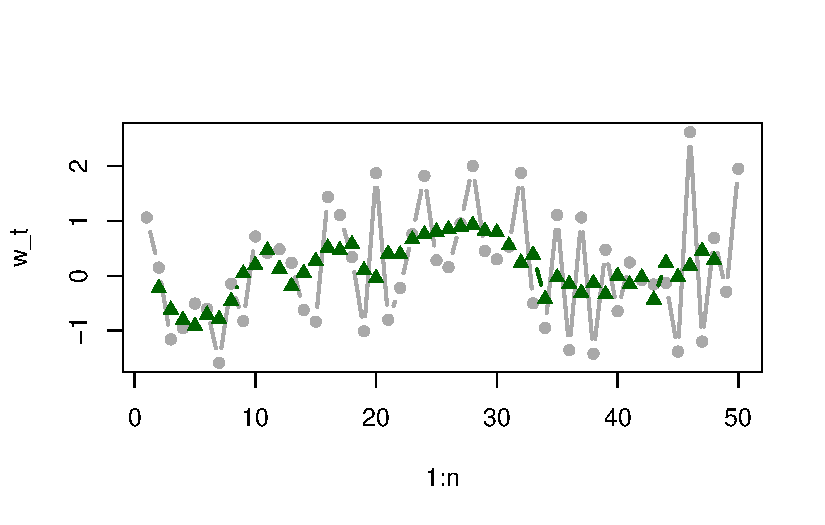
\includegraphics{LectureNotes/Lecture2_files/figure-pdf/unnamed-chunk-14-2.pdf}

\chapter{Problem 1.1}\label{problem-1.1}

\section{Moving Averages (Problem
1.1)}\label{moving-averages-problem-1.1}

\begin{itemize}
\tightlist
\item
  using a method similar to the code in Example 1.9, generate 100
  observations from the autoregression \[
  x_t = -0.9x_{t-2} + w_t\text{, }\\ w_t\sim N(0, 1)
  \]
\item
  Write down an expression for \(\phi\) for this autoregression. How is
  \(\phi\) different from the autoregression in Example 1.9?
\end{itemize}

\section{Moving Averages (Problem 1.1 Part
a)}\label{moving-averages-problem-1.1-part-a}

\begin{itemize}
\item
  Apply the moving average filter to the autoregression data you
  generated \[
  v_t = (x_t + x_{t-1} + x_{t-2} + x_{t-4})
  \]
\item
  Plot \(x_t\) as points and lines and \(v_t\) as a line.
\end{itemize}

\section{Moving Averages (Problem
1.1)}\label{moving-averages-problem-1.1-1}

\begin{Shaded}
\begin{Highlighting}[]
\FunctionTok{library}\NormalTok{(astsa)}
\NormalTok{w }\OtherTok{=} \FunctionTok{rnorm}\NormalTok{(}\DecValTok{150}\NormalTok{,}\DecValTok{0}\NormalTok{,}\DecValTok{1}\NormalTok{) }\CommentTok{\# 50 extra to avoid startup problems}
\NormalTok{xa }\OtherTok{=} \FunctionTok{filter}\NormalTok{(w, }\AttributeTok{filter=}\FunctionTok{c}\NormalTok{(}\DecValTok{0}\NormalTok{,}\SpecialCharTok{{-}}\NormalTok{.}\DecValTok{9}\NormalTok{), }\AttributeTok{method=}\StringTok{"recursive"}\NormalTok{)[}\SpecialCharTok{{-}}\NormalTok{(}\DecValTok{1}\SpecialCharTok{:}\DecValTok{50}\NormalTok{)] }\CommentTok{\# AR}
\NormalTok{va }\OtherTok{=} \FunctionTok{filter}\NormalTok{(xa, }\FunctionTok{rep}\NormalTok{(}\DecValTok{1}\NormalTok{,}\DecValTok{4}\NormalTok{)}\SpecialCharTok{/}\DecValTok{4}\NormalTok{, }\AttributeTok{sides=}\DecValTok{1}\NormalTok{) }\CommentTok{\# moving average}
\FunctionTok{tsplot}\NormalTok{(xa, }\AttributeTok{main=}\StringTok{"autoregression"}\NormalTok{, }\AttributeTok{type =} \StringTok{"b"}\NormalTok{, }\AttributeTok{pch =} \DecValTok{16}\NormalTok{)}
\FunctionTok{lines}\NormalTok{(va, }\AttributeTok{col=}\StringTok{"blueviolet"}\NormalTok{, }\AttributeTok{lwd =} \DecValTok{2}\NormalTok{)}
\end{Highlighting}
\end{Shaded}

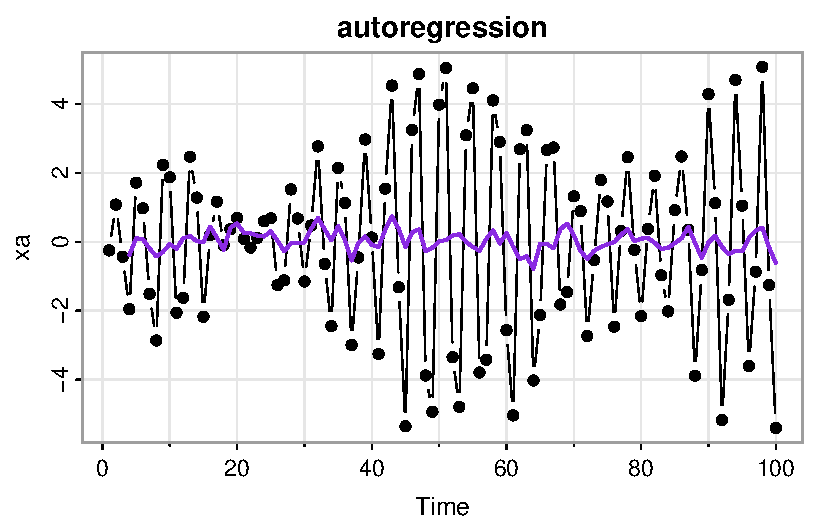
\includegraphics{LectureNotes/Lecture2_files/figure-pdf/unnamed-chunk-15-1.pdf}

\section{Moving Averages (Problem 1.1 part
b)}\label{moving-averages-problem-1.1-part-b}

\begin{itemize}
\tightlist
\item
  Repeat the application of the MA filter but instead of starting with
  an autoregression, generate data \(x_t\) according to the signal plus
  noise model \[
  x_t = 2\cos(2\pi t/4) + w_t\\ w_t \sim N(0,1)
  \]
\end{itemize}

\section{Moving Averages (Problem 1.1 part
b)}\label{moving-averages-problem-1.1-part-b-1}

\begin{Shaded}
\begin{Highlighting}[]
\NormalTok{xb }\OtherTok{=} \DecValTok{2}\SpecialCharTok{*}\FunctionTok{cos}\NormalTok{(}\DecValTok{2}\SpecialCharTok{*}\NormalTok{pi}\SpecialCharTok{*}\NormalTok{(}\DecValTok{1}\SpecialCharTok{:}\DecValTok{100}\NormalTok{)}\SpecialCharTok{/}\DecValTok{4}\NormalTok{) }\SpecialCharTok{+} \FunctionTok{rnorm}\NormalTok{(}\DecValTok{100}\NormalTok{,}\DecValTok{0}\NormalTok{,}\DecValTok{1}\NormalTok{) }\CommentTok{\# sinusoid + noise}
\NormalTok{vb }\OtherTok{=} \FunctionTok{filter}\NormalTok{(xb, }\FunctionTok{rep}\NormalTok{(}\DecValTok{1}\NormalTok{,}\DecValTok{4}\NormalTok{)}\SpecialCharTok{/}\DecValTok{4}\NormalTok{, }\AttributeTok{sides=}\DecValTok{1}\NormalTok{) }\CommentTok{\# moving average}
\FunctionTok{tsplot}\NormalTok{(xb, }\AttributeTok{main=}\StringTok{"sinusoid + noise"}\NormalTok{, }\AttributeTok{type =} \StringTok{"b"}\NormalTok{, }\AttributeTok{pch =} \DecValTok{16}\NormalTok{)}
\FunctionTok{lines}\NormalTok{(vb, }\AttributeTok{col=}\StringTok{"blueviolet"}\NormalTok{, }\AttributeTok{lwd =} \DecValTok{2}\NormalTok{)}
\end{Highlighting}
\end{Shaded}

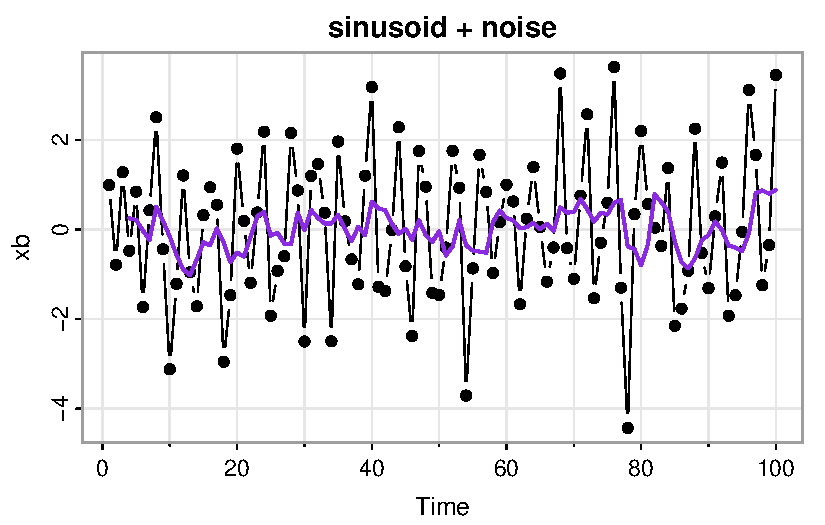
\includegraphics{LectureNotes/Lecture2_files/figure-pdf/unnamed-chunk-16-1.pdf}

\section{Moving Averages (Problem 1.1 part
c)}\label{moving-averages-problem-1.1-part-c}

\begin{itemize}
\tightlist
\item
  Repeat the application of the MA filter but instead of starting with
  an autoregression, use the Johnson and Johnson data from Lecture 1.
\end{itemize}

\section{Moving Averages (Problem 1.1 part
c)}\label{moving-averages-problem-1.1-part-c-1}

\begin{Shaded}
\begin{Highlighting}[]
\NormalTok{xc }\OtherTok{=} \FunctionTok{log}\NormalTok{(jj)}
\NormalTok{vc }\OtherTok{=}\NormalTok{ stats}\SpecialCharTok{::}\FunctionTok{filter}\NormalTok{(xc, }\AttributeTok{filter =} \FunctionTok{rep}\NormalTok{(}\DecValTok{1}\NormalTok{,}\DecValTok{4}\NormalTok{)}\SpecialCharTok{/}\DecValTok{4}\NormalTok{, }\AttributeTok{sides=}\DecValTok{1}\NormalTok{, }\AttributeTok{method =} \StringTok{"convolution"}\NormalTok{) }\CommentTok{\# moving average}
\FunctionTok{tsplot}\NormalTok{(xc, }\AttributeTok{main=}\StringTok{"johnson and johnson (log scale)"}\NormalTok{, }\AttributeTok{type =} \StringTok{"b"}\NormalTok{, }\AttributeTok{pch =} \DecValTok{16}\NormalTok{)}
\FunctionTok{lines}\NormalTok{(vc, }\AttributeTok{col=}\StringTok{"blueviolet"}\NormalTok{, }\AttributeTok{lwd =} \DecValTok{2}\NormalTok{)}
\end{Highlighting}
\end{Shaded}

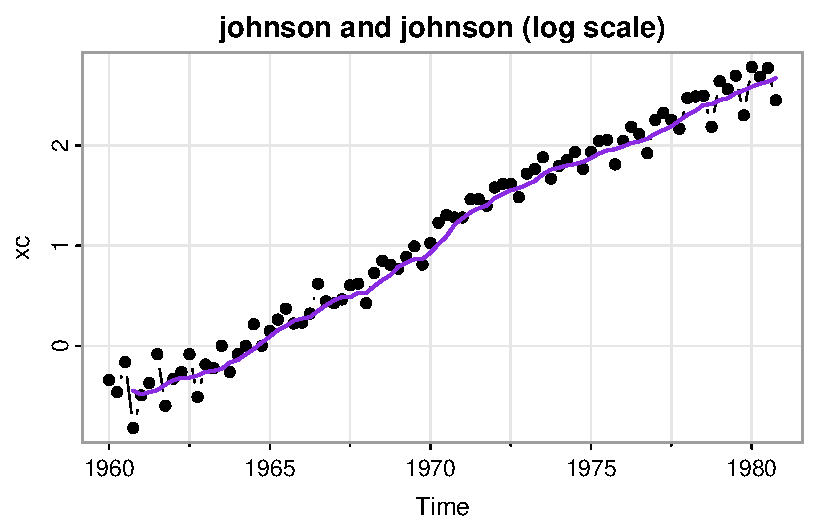
\includegraphics{LectureNotes/Lecture2_files/figure-pdf/unnamed-chunk-17-1.pdf}

\section{Stationarity}\label{stationarity}

A time series is stationary if

\begin{itemize}
\tightlist
\item
  the mean function (\(\mu_t\)) is constant and does not depend on time
  \(t\)
\item
  the autocovariance function (\(\gamma(s,t)\)) depends on \(s\) and
  \(t\) only though their difference
\end{itemize}

\section{Example 2.14 Stationarity of a Random
Walk}\label{example-2.14-stationarity-of-a-random-walk}

Look, it's our friend the random walk:

\[
x_t = \delta t + \sum_{j = 1}^t w_j
\] Their mean function is \(\E(x_t) = 0\), and their covariance function
is \(\gamma_x(s, t) = \min\{s,t\}\sigma^2_w\)

Is a random walk stationary?

\chapter{Stat 416 Assignment 1 Due Monday, September 30 at
11:59:59PM}\label{stat-416-assignment-1-due-monday-september-30-at-115959pm}

A paper I worked on as a research scientist considered the time series
of the concentration (measured as \(\log_{10}\) copies per Liter) of the
SARS-CoV-2 virus from 5 different locations in the City of Houston,
visualized in parts (c)-(g) of the figure below.

The goal of this study was to see whether the information gleaned from
sampling the lift stations, which represent smaller populations, was
different than the information gleaned from sampling only the larger
wastewater treatment plant. In other words, one research question was to
determine whether the WWTP (dark blue) time series has different
dynamics (behavior) than those that represent the lift stations.

The methods in this paper are touched on in chapter 8 of our textbook.
For this assignment, we will use the wastewater data as an example and
practice our plotting and time series data science skills.

\begin{figure}[H]

{\centering \includegraphics{index_files/mediabag/41598_2024_56175_Fig.png}

}

\caption{(a) The WWTP catchment areas for the City of Houston, with the
WWTP of focus shaded. The box shows the extent of (b), the map showing
the 4 lift stations considered in the analysis. (c--g) Plot the time
series of Log10 Copies/L for the WWTP and the 4 lift station facilities,
referred to as Lift Station A--D, with periods of missing values
indicated by grey rectangles.}

\end{figure}%

\begin{enumerate}
\def\labelenumi{\arabic{enumi}.}
\item
  {[}6 points{]} Which of the time series has the most missing data?
  Which appears to have the most variability? Does the overall behavior
  of the series seem to be similar?
\item
  {[}5 points{]} Load the (synthetic) wastewater data from
  \url{https://raw.githubusercontent.com/hou-wastewater-epi-org/online_trend_estimation/refs/heads/main/Data/synthetic_ww_time_series.csv}
  using the \texttt{read.csv} function

\begin{Shaded}
\begin{Highlighting}[]
\NormalTok{ww }\OtherTok{\textless{}{-}} \FunctionTok{read.csv}\NormalTok{(}\CommentTok{\#your code here)}
\end{Highlighting}
\end{Shaded}
\item
  {[}5 points{]} Inspect the data. Verify that each of the series from
  the map above are included in the .csv (hint: what are the unique
  values of the \texttt{name} field?)

\begin{Shaded}
\begin{Highlighting}[]
\CommentTok{\#your code here}
\end{Highlighting}
\end{Shaded}
\item
  {[}5 points{]} Convert the date field to a Date format using the
  function as.Date.

\begin{Shaded}
\begin{Highlighting}[]
\NormalTok{ww}\SpecialCharTok{$}\NormalTok{dates }\OtherTok{\textless{}{-}} \FunctionTok{as.Date}\NormalTok{(}\CommentTok{\# your code here)}
\end{Highlighting}
\end{Shaded}
\item
  {[}2 points{]} Install and load the \texttt{tidyverse} package.

\begin{Shaded}
\begin{Highlighting}[]
\DocumentationTok{\#\# your code here}
\end{Highlighting}
\end{Shaded}
\item
  {[}5 points{]} We will work with just the WWTP series for now. Use
  \texttt{dplyr::filter} to extract the values for just the WWTP series.

\begin{Shaded}
\begin{Highlighting}[]
\NormalTok{ww\_WWTP }\OtherTok{\textless{}{-}}\NormalTok{ ww }\SpecialCharTok{\%\textgreater{}\%}\NormalTok{ dplyr}\SpecialCharTok{::}\FunctionTok{filter}\NormalTok{(}\CommentTok{\#your code here)}
\end{Highlighting}
\end{Shaded}
\item
  {[}10 points{]} What is the time interval between the observations?
  How do you know?
\item
  {[}10 points total{]} Use the \texttt{tsplot} function from the
  \texttt{astsa} package to plot the \texttt{WWTP} series {[}5
  points{]}.

  Make sure to use the \texttt{dates} {[}2 points{]}field for the x-axis
  and specify good axis and plot labels using the
  \texttt{xlab}/\texttt{ylab}, and \texttt{main} arguments {[}1 point
  each{]}. (see the documentation \texttt{?tsplot} for more)

\begin{Shaded}
\begin{Highlighting}[]
\DocumentationTok{\#\# your code here}
\end{Highlighting}
\end{Shaded}
\item
  {[}10 points{]} Apply a moving average filter with 3 time points using
  the stats::filter function and save the result in a vector called
  \texttt{ww\_ma\_3}. (Similar to the final part of problem 1.1, see
  \href{http://localhost:4512/LectureNotes/Lecture2.html\#moving-averages-problem-1.1-part-c}{here}
  in Lecture Notes).

\begin{Shaded}
\begin{Highlighting}[]
\FunctionTok{library}\NormalTok{(astsa)}
\NormalTok{ww\_ma\_3 }\OtherTok{\textless{}{-}}\NormalTok{ stats}\SpecialCharTok{::}\FunctionTok{filter}\NormalTok{(}\CommentTok{\#your code here)}
\end{Highlighting}
\end{Shaded}
\item
  {[}10 points{]} Plot the moving average you computed on top of the
  tsplot in a different color using the lines function (see linked
  Problem 1.1 above). In the call to the lines function, also use
  \texttt{type\ =\ l} and \texttt{lwd\ =\ 2}.

\begin{Shaded}
\begin{Highlighting}[]
\FunctionTok{tsplot}\NormalTok{(}\CommentTok{\# your code here)}
\FunctionTok{lines}\NormalTok{(}\CommentTok{\# your code here)}
\end{Highlighting}
\end{Shaded}
\item
  {[}15 points{]} Apply the moving average filter again, but this time
  use 5 time points, call it \texttt{ww\_ma\_5}. Plot just the
  \texttt{WWTP} series data and the \texttt{ww\_ma\_5} you just
  computed, and use a different color for this MA process than you used
  in question 10.

\begin{Shaded}
\begin{Highlighting}[]
\DocumentationTok{\#\# your code here (similar to part 9 and 10, but with 5 time points)}
\end{Highlighting}
\end{Shaded}
\item
  {[}5 points{]} Inspect the plot you generated in questions 10 and 11.
  Which MA process looks ``smoother''?
\item
  {[}10 points{]} Describe the different way that the missing data in
  the WWTP series impacts the moving average estimates for the case of 3
  time points vs.~5 time points.
\item
  {[}5 points{]} Note that the data you used for this activity was
  ``synthetic'' wastewater data. Why might a researcher share a
  synthetic version of their data? What do you think that might mean?
\end{enumerate}



\end{document}
